\documentclass[11pt, twoside, pdftex]{article}

% This include all the settings that we should use for the document
\newcommand{\PDFTitle}{Introduction to the Intel\textsuperscript{\textregistered} Nios\textsuperscript{\textregistered} II Soft Processor}
\newcommand{\commonPath}{../../Common}
\newcommand{\datePublished}{Mar 2022}

\newcommand{\versnum}{21.1} %version number quartus/AMP
\newcommand{\quartusname}{Quartus\textsuperscript{\textregistered} Prime}	
\newcommand{\textBar}{For \quartusname{} \versnum{}}
\newcommand{\thisyear}{2022 } %for copyright
\newcommand{\company}{FPGAcademy.org}
\newcommand{\longteamname}{FPGAcademy.org}
\newcommand{\teamname}{FPGAcademy}
\newcommand{\website}{FPGAcademy.org}

\newcommand{\productAcronym}{AMP}
\newcommand{\productNameShort}{Monitor Program}

\newcommand{\productNameMedTM}{Monitor Program}
\newcommand{\productNameMed}{Monitor Program}

%\newcommand{\headerLogoFilePath}[1]{#1/FPGAcademy.png}



\setlength\topmargin{-0.25in}
\setlength\headheight{0in}
\setlength\headsep{0.35in}
\setlength\textheight{8.5in}
\setlength\textwidth{7in}
\setlength\oddsidemargin{-0.25in}
\setlength\evensidemargin{-0.25in}
\setlength\parindent{0.25in}
\setlength\parskip{0in} 

\pdfpagewidth 8.5in
\pdfpageheight 11in

% listings is a package that supports encapsulating source code in LaTeX conveniently

\usepackage{listings}
% add support for graphics
\usepackage{graphicx}
\usepackage[usenames, dvipsnames]{color}

\def\expandparam\lstinputlisting[#1]#2{\edef\tmp{\noexpand\lstinputlisting[#1]{#2}}\tmp}

\widowpenalty 10000
\clubpenalty 10000

%%%%%%%%%%%%%%%%%%%% Source Code Formatting %%%%%%%%%%%%%%%%%%%%
\definecolor{globalCommentColour}{rgb}{0.588,0.588,0.588}

%%%%%%%%%%%%%%%%%%%%%%%%%%%%%%%%%%%%%%%%%%%%%%%%%%%%
% Defining a NiosII ASM highlighter for lstlisting
\lstdefinelanguage[NiosII]{Assembler} {
 	morekeywords={add, addi, and, andhi, andi, beq, bge, bgeu, bgt, bgtu, ble,  bleu, blt, bltu, bne, br, break,% 
 	bret, call, callr, cmpeq, cmpeqi, cmpge, cmpgei, cmpgeu, cmpgeui, cmpgt, cmpgti, cmpgtu, cmpgtui, cmple,%
 	cmplei, cmpleu, cmpleui, cmplt, cmplti, cmpltu, cmpltui, cmpne, cmpnei, custom, div, divu, eret, flushd,%
 	flushda, flushi, flushp, initd, initda, initi, jmp, jmpi, ldb, ldbio, ldbu, ldbuio, ldh, ldhio, ldhu, ldhuio,%
 	ldw, ldwio, mov, movhi, movi, movia, movui, mul, muli, mulxss, mulxsu, mulxuu, nextpc, nop, nor, or, orhi, ori,%
 	rdctl, rdprs, ret, rol, roli, ror, sll, slli, sra, srai, srl, srli, stb, stbio, sth, sthio, stw, stwio,%
 	sub, subi, sync, trap, wrctl, wrtcl, wrprs, xor, xori, xorhi, xori},% 	
 	morekeywords=[2]{.abort, .ABORT, .align, .app-file, .ascii, .asciz, .balign, .byte, .comm, .data, .def,%
 	.desc, .dim, .double, .eject, .else, .end, .endef, .endif, .equ, .equiv, .err, .extern, .file, .fill, .float,%
 	.global, .globl, .hword, .ident, .if, .include, .int, .irp, .irpc, .lcomm, .lflags, .line, .linkonce, .ln,%
 	.list, .long, .macro, .mri, .nolist, .octa, .org, .p2align, .psize, .quad, .rept, .sbttl, .scl, .section,%
 	.set, .short, .single, .size, .sleb128, .skip, .space, .stadb, .stabn, .stabs, .string, .symver, .tag,%
 	.text, .title, .type, .val, .uleb128, .word},% 	
 	morekeywords=[3]{et, bt, gp, sp, fp, ea, sstatus, ra, pc, status, estatus, bstatus, ienable, ipending, cpuid,%
 	exception, pteaddr, tlbacc, tlbmisc, eccinj, badaddr, config, mpubase, mpuacc},% 	
 	sensitive=t,%
 	alsoletter=.,%
	morestring=[b]",%
 	morecomment=[s]{/*}{*/},%
 	morecomment=[l]\#,%
   }[keywords,comments,strings]
   
   %% NOTE: morekeywords=[2] are GNU directives.
   
   \definecolor{niosInstructionColour}{rgb}{0.000,0.608,0.000}
   \definecolor{niosDirectiveColour}{rgb}{0.000,0.000,0.902}
   \definecolor{niosSpecialRegColour}{rgb}{0.000,0.000,0.000}
   \definecolor{niosStringColour}{rgb}{0.808,0.482,0.000}
   
   %% NOTE: To make bold use: =\bfseries\color{<colour>}
   \lstdefinestyle{defaultNiosStyle} {
   language=[NiosII]{Assembler},
   stringstyle=\color{niosStringColour},
   keywordstyle=\color{niosInstructionColour},
   keywordstyle=[2]\color{niosDirectiveColour},
   keywordstyle=[3]\itshape\color{niosSpecialRegColour}
   }
%%%%%%%%%%%%%%%%%%%%%%%%%%%%%%%%%%%%%%%%%%%%%%%%%%%%

%%%%%%%%%%%%%%%%%%%%%%%%%%%%%%%%%%%%%%%%%%%%%%%%%%%%
% Defining a ArmA9 ASM highlighter for lstlisting
\lstdefinelanguage[ArmA9]{Assembler} {
 	morekeywords={ADC, ADD, ADDS, AND, ANDS, B, BAL, BEQ, BGE, BGT, BL, BLT, BIC, BKPT, BLX, BNE, BX, CDP, CLZ, CMN, CMP, EOR,%
 	EORS, LDC, LDM, LDR, LDRB, LDRBT, LDRH, LDRSB, LDRSH, LDRT, LSL, MCR, MLA, MOV, MOVW, MOVT, MRC, MRS, MSR, MUL, MVN, ORR, PLD,%
 	ROR, RSB, RSC, SBC, SMLAL, SMULL, STC, STM, STR, STRB, STRBT, STRH, STRT, SUB, SUBS, SWI, SWP, SWPB, TEQ, UMLAL,
 	PUSH, POP, MOVS, RORS, LSR},%
 	morekeywords=[2]{.abort, .ABORT, .align, .app-file, .ascii, .asciz, .balign, .byte, .comm, .data, .def,%
 	.desc, .dim, .double, .eject, .else, .end, .endef, .endif, .equ, .equiv, .err, .extern, .file, .fill, .float,%
 	.global, .globl, .hword, .ident, .if, .include, .int, .irp, .irpc, .lcomm, .lflags, .line, .linkonce, .ln,%
 	.list, .long, .macro, .mri, .nolist, .octa, .org, .p2align, .psize, .quad, .rept, .sbttl, .scl, .section,%
 	.set, .short, .single, .size, .sleb128, .skip, .space, .stadb, .stabn, .stabs, .string, .symver, .tag,%
 	.text, .title, .type, .val, .vectors, .uleb128, .word},%
 	morekeywords=[3]{SP, PC, MIDR, CTR, TCMTR, TLBTR, MPIDR, ID_PFR0, ID_PFR1, ID_DFR0, ID_MMFR0, ID_MMFR1, ID_MMFR2,%
 	ID_MMFR3, ID_ISAR0, ID_ISAR1, ID_ISAR2, ID_ISAR3, ID_ISAR4, CCSIDR, CLIDR, AIDR, CSSELR, TTBR0, TTRB1, TTBR2, DACR,%
 	DFSR, IFSR, ADFSR, AIFSR, DFAAR, IFAR, ICIALLUIS, BPIALLIS, PAR, ICIALLU, ICIMVAU, BPIALL, DCIMVAC, DCISW, V2PCWPR,%
 	DCCVAC, DCCSW, DDIMVAC, DCISW, TLBALLIS, TLBIMVAIS, TLBIASIDIS, TLBIMVAAIS, TLBIALL, TLBIMVA, TLBIASID, TLBIMVAA,%
 	PMCR, PMCNTENSET, PMCNTENCLR, PMOVSR, PMSWINC, PMSELR, PMXEVTYPER, PMXEVCNTR, PMUSERENR, PMINTENSET, PMINTENCLR,%
 	PRRR, NRRR, PLEIDR, PLEASR, PLEFSR, PLEUAR, PLEPCR, VBAR, MVBAR, ISR, FCSEIDR, CONTEXTIDR, TPIDRURW, TPIDRURO, TPIDRPRW},%
 	sensitive=f,%
 	alsoletter=.,%
	morestring=[b]",%
 	morecomment=[s]{/*}{*/},%
 	morecomment=[l]{//},%
   }[keywords,comments,strings]
   
   %% NOTE: morekeywords=[2] are GNU directives.
   
   \definecolor{armInstructionColour}{rgb}{0.000,0.608,0.000}
   \definecolor{armDirectiveColour}{rgb}{0.000,0.000,0.902}
   \definecolor{armSpecialRegColour}{rgb}{0.000,0.000,0.000}
   \definecolor{armStringColour}{rgb}{0.808,0.482,0.000}
   
   \lstdefinestyle{defaultArmStyle} {
   language=[ArmA9]{Assembler},
   stringstyle=\color{armStringColour},
   keywordstyle=\color{armInstructionColour},
   keywordstyle=[2]\color{armDirectiveColour},
   keywordstyle=[3]\itshape\color{armSpecialRegColour}
   }
%%%%%%%%%%%%%%%%%%%%%%%%%%%%%%%%%%%%%%%%%%%%%%%%%%%%

%%%%%%%%%%%%%%%%%%%%%%%%%%%%%%%%%%%%%%%%%%%%%%%%%%%%
% Defining style for the verilog.

\definecolor{verilogCommentColour}{rgb}{0.000,0.502,0.000}

\lstdefinestyle{defaultVerilogStyle} {
language={Verilog},
keywordstyle=\color{blue},
commentstyle=\color{verilogCommentColour}
}
%%%%%%%%%%%%%%%%%%%%%%%%%%%%%%%%%%%%%%%%%%%%%%%%%%%%

%%%%%%%%%%%%%%%%%%%%%%%%%%%%%%%%%%%%%%%%%%%%%%%%%%%%
% Defining style for the vhdl.
\lstdefinestyle{defaultVHDLStyle} {
language={VHDL},
keywordstyle=\color{blue},
commentstyle=\color{verilogCommentColour}
}
%%%%%%%%%%%%%%%%%%%%%%%%%%%%%%%%%%%%%%%%%%%%%%%%%%%%

%%%%%%%%%%%%%%%%%%%%%%%%%%%%%%%%%%%%%%%%%%%%%%%%%%%%
% Java
\definecolor{javaStringColour}{rgb}{0.808,0.482,0}
%%%%%%%%%%%%%%%%%%%%%%%%%%%%%%%%%%%%%%%%%%%%%%%%%%%%

%%%%%%%%%%%%%%%%%%%%%%%%%%%%%%%%%%%%%%%%%%%%%%%%%%%%
% Defining language styles
% C
\definecolor{CStringColour}{rgb}{0.808,0.482,0}
%%%%%%%%%%%%%%%%%%%%%%%%%%%%%%%%%%%%%%%%%%%%%%%%%%%%

%%%%%%%%%%%%%%%%%%%%%%%%%%%%%%%%%%%%%%%%%%%%%%%%%%%%
% Defining extended LaTeX language.
\lstdefinelanguage[LocalLaTeX]{TeX}[LaTeX]{TeX}%
 	{moretexcs={bf, it, sf, lstset},%
   	}%

\lstdefinestyle{defaultLocalLatexStyle} {
language=[LocalLatex]{TeX},
keywordstyle=\color{blue}\bfseries,
keywordstyle=[2]\color{blue},
keywordstyle=[3]\color{blue}\bfseries
}
%%%%%%%%%%%%%%%%%%%%%%%%%%%%%%%%%%%%%%%%%%%%%%%%%%%%

\lstset{
%language = C,
%language = Verilog,
%basicstyle=\color{black}\rmfamily\ttfamily,
basicstyle=\small\color{black}\ttfamily,
commentstyle=\small\color{globalCommentColour}\itshape\ttfamily,
keywordstyle=\small\color{blue}\bfseries\ttfamily,
showstringspaces=false,
frame=none, %lines % boxed listings
breaklines=true,
breakatwhitespace=true,
tabsize=4
}
%%%%%%%%%%%%%%%%%%%%%%%%%%%%%%%%%%%%%%%%%%%%%%%%%%%%%%%%%%%%%%%%


%\usepackage[centering]{geometry}.
%%%%%%%%%%%%%%%%%%%%%%%%%%%%%%%%%%%%%%%%%%%%%%%%%%%
% Document Settings
\usepackage[labelsep=period]{caption}
% we can choose a better font later
%\usepackage{palatino}
\usepackage{fourier}
%\fontencoding{T1}
% include common used symbols
\usepackage{textcomp}
% add support for graphics
\usepackage{graphicx}
\usepackage[usenames, dvipsnames]{color}
% enable to draw thick or thin table hlines
\setlength{\doublerulesep}{\arrayrulewidth}
\usepackage{longtable}
\setlongtables
%\usepackage{array}
% It may be better to use PDFLaTeX as it can generate bookmarks for the
% document

% Add some useful packages
\usepackage{ae,aecompl}
\usepackage{epsfig,float,times}

% reset the font for section
\usepackage{sectsty}
%\allsectionsfont{\fontfamily{ptm}\selectfont}
\allsectionsfont{\usefont{OT1}{phv}{bc}{n}\selectfont}

% use compact space for sections
\usepackage[compact]{titlesec}
\titlespacing{\section}{0pt}{0.2in}{*0}
\titlespacing{\subsection}{0pt}{0.1in}{*0}
\titlespacing{\subsubsection}{0pt}{0.05in}{*0}

% fancyhdr header and footer customization
\usepackage{layout}
\usepackage{fancyhdr}
\pagestyle{fancy}
\fancyhead{}
\fancyhead[R]{\textit{\tiny{\textBar}}}
\fancyfoot{}
\fancyfoot[LO,
RE]{\textrm{\href{https://www.fpgacademy.org}{\small \longteamname}} \\ {\small \datePublished }}
\fancyfoot[RO, LE]{\small \thepage}
% two-side settings
%\fancyhead{} % clear all header fields
%\fancyfoot{} % clear all footer fields
%\fancyfoot[LE,RO]{\thepage}
\renewcommand{\headrulewidth}{2pt}
\renewcommand{\headrule}{{\color{blue} \hrule width\headwidth height\headrulewidth \vskip-\headrulewidth}}
\renewcommand{\footrulewidth}{0pt}

% Format the footer on page 1
\fancypagestyle{plain}{
\fancyhead{}
\fancyfoot{}
\fancyfoot[LO,
RE]{\textrm{\href{https://www.fpgacademy.org}{\small \longteamname}} \\ {\small \datePublished }}
\fancyfoot[RO, LE]{\small \thepage}
\renewcommand{\headrulewidth}{0pt}
}
% adjust some setting to try to make the figure stay in the same page with text
% Reference: 	http://www.cs.uu.nl/~piet/floats/node1.html
%   			http://mintaka.sdsu.edu/GF/bibliog/latex/floats.html
%   General parameters, for ALL pages:
\renewcommand{\topfraction}{0.9}	% max fraction of floats at top
\renewcommand{\bottomfraction}{0.8}	% max fraction of floats at bottom
%   Parameters for TEXT pages (not float pages):
\setcounter{topnumber}{3}
\setcounter{bottomnumber}{3}
\setcounter{totalnumber}{5}     % 2 may work better
\setcounter{dbltopnumber}{2}    % for 2-column pages
\renewcommand{\dbltopfraction}{0.9}	% fit big float above 2-col. text
\renewcommand{\textfraction}{0.07}	% allow minimal text w. figs
%   Parameters for FLOAT pages (not text pages):
\renewcommand{\floatpagefraction}{0.7}	% require fuller float pages
% N.B.: floatpagefraction MUST be less than topfraction !!
\renewcommand{\dblfloatpagefraction}{0.7}	% require fuller float pages
%%%%%%%%%%%%%%%%%%%%%%%%%%%%%%%%%%%%%%%%%%%%%%%%%%%
% remember to use [htp] or [htpb] for placement
%%%%%%%%%%%%%%%%%%%%%%%%%%%%%%%%%%%%%%%%%%%%%%%%%%%

% set no indent for paragraph
\setlength{\parindent}{0em}
\addtolength{\parskip}{11pt}
\newcommand{\compact}{[topsep=0pt]}
% use this package to reduce space
\usepackage{enumitem}
\usepackage{multirow}
\usepackage{rotating}
\usepackage{pifont}
\usepackage{dingbat}
\newcommand{\itemsecond}{$\circ$}
%
%%%%%%%%%%%%%%%%%%
\date{}
\author{}
%%%%%%%%%%%%%%%%%%
\newcommand{\de}{DE-series}
\newcommand{\up}{FPGAcademy}
\newcommand{\fabric}{Avalon Switch Fabric}
\newcommand{\TODO}[1]{\textcolor{red}{\textbf{TODO}: #1}}
\def\registered{{\ooalign{\hfil\raise .00ex\hbox{\scriptsize R}\hfil\crcr\mathhexbox20D}}}

% enable url and reference(bookmarks) in pdf
\usepackage{url}
\usepackage[pdftex, colorlinks]{hyperref}
\hypersetup{%
pdftitle={\PDFTitle},
linkcolor=blue,
hyperindex=true,
pdfauthor={\longteamname},
pdfkeywords={FPGAcademy, Academic Program, Example System},
bookmarksnumbered,
bookmarksopen=false,
filecolor=blue,
pdfstartview={FitH},
urlcolor=blue,
plainpages=false,
pdfpagelabels=true,
linkbordercolor={1 1 1} %no color for link border
}%
%%%%%%%%%%%%%%%%%%%%%%%%%%%%%%%%%%%%%%%%%%%%%%%%%%%
\setlength{\fboxsep}{0.7pt}
\setlength{\fboxrule}{0.5pt}

\newcommand{\red}[1]{{\color{red}\sf{#1}}}
\newcommand{\blue}[1]{{\color{blue}\sf{#1}}}



%%%%%%%%%%%%%%%%%%%%%%%%%
% Add title
\newcommand{\doctitle}{Introduction to the Intel\textsuperscript{\textregistered} \\ Nios\textsuperscript{\textregistered} II Soft Processor}
\newcommand{\dochead}{Introduction to the Intel\textsuperscript{\textregistered} Nios\textsuperscript{\textregistered} II Soft Processor}
% Usually no need to change these two lines
\title{\fontfamily{phv}\selectfont{\doctitle} }
\chead{ \small{\textsc{\bfseries \dochead} } }
% Customizations
%%%%%%%%%%%%%%%%%%%%%%%%%
% Allows multiple figures per page

\renewcommand\floatpagefraction{.9}
\renewcommand\topfraction{.9}
\renewcommand\bottomfraction{.9}
\renewcommand\textfraction{.1}   
\setcounter{totalnumber}{50}
\setcounter{topnumber}{50}
\setcounter{bottomnumber}{50}
\raggedbottom

%%%%%%%%%%%%%%%%%%
%%% DOCUMENT START
%\begin{document}
\begin{document}
\begin{table}
    \centering
    \begin{tabular}{p{5cm}p{4cm}}
        \hspace{-3cm}
        &
        \raisebox{1\height}{\parbox[h]{0.5\textwidth}{\Large\fontfamily{phv}\selectfont{\textsf{\doctitle}}}}
    \end{tabular}
    \label{tab:logo}
\end{table}

\colorbox[rgb]{0,0.384,0.816}{\parbox[h]{\textwidth}{\color{white}\textsf{\textit{\textBar}}}}

\thispagestyle{plain}
 
\section{Introduction}

This tutorial presents an introduction the Intel\textsuperscript{\textregistered} Nios\textsuperscript{\textregistered} II processor, 
which is a soft processor that can be instantiated on an Intel FPGA device.
It describes the basic architecture of Nios II and its instruction set.
The Nios II processor and its associated memory and peripheral components are
easily instantiated by using Intel's SOPC Builder or Platform Designer tool in conjunction with the 
Quartus\textsuperscript{\textregistered} Prime software. 

A full description of the Nios II processor is provided in the 
{\it Nios II Processor Reference Handbook}, which is available in the literature
section of the Intel web site. Introductions to the SOPC Builder and Platform Designer tools are given in the tutorials {\it Introduction to the Intel SOPC Builder} and 
{\it Introduction to the Intel Platform Designer Tool}, respectively.  Both can be found in the University Program section of the web site.

{\bf Contents}:
\begin{itemize}
\item Nios II System
\item Overview of Nios II Processor Features
\item Register Structure
\item Accessing Memory and I/O Devices
\item Addressing
\item Instruction Set
\item Assembler Directives
\item Example Program
\item Exception Processing
\item Cache Memory
\item Tightly Coupled Memory
\end{itemize}
\clearpage
\newpage

\section{Background}

Intel's Nios II is a soft processor, defined in a hardware description language,
which can be implemented in Intel's FPGA devices by using the 
Quartus Prime CAD system. 
This tutorial provides a basic introduction to the Nios II processor, intended for
a user who wishes to implement a Nios II based system on an Intel Development and 
Education board.

\section{Nios II System}
The Nios II processor can be used with a variety of other components to form 
a complete system. These components include a number of standard peripherals, 
but it is also possible to define custom peripherals. Intel's DE-series boards
contain several components that can be integrated
into a Nios II system. An example of such a system is shown in Figure~\ref{fig:1}.
 
\begin{figure}[H]
   \begin{center}
      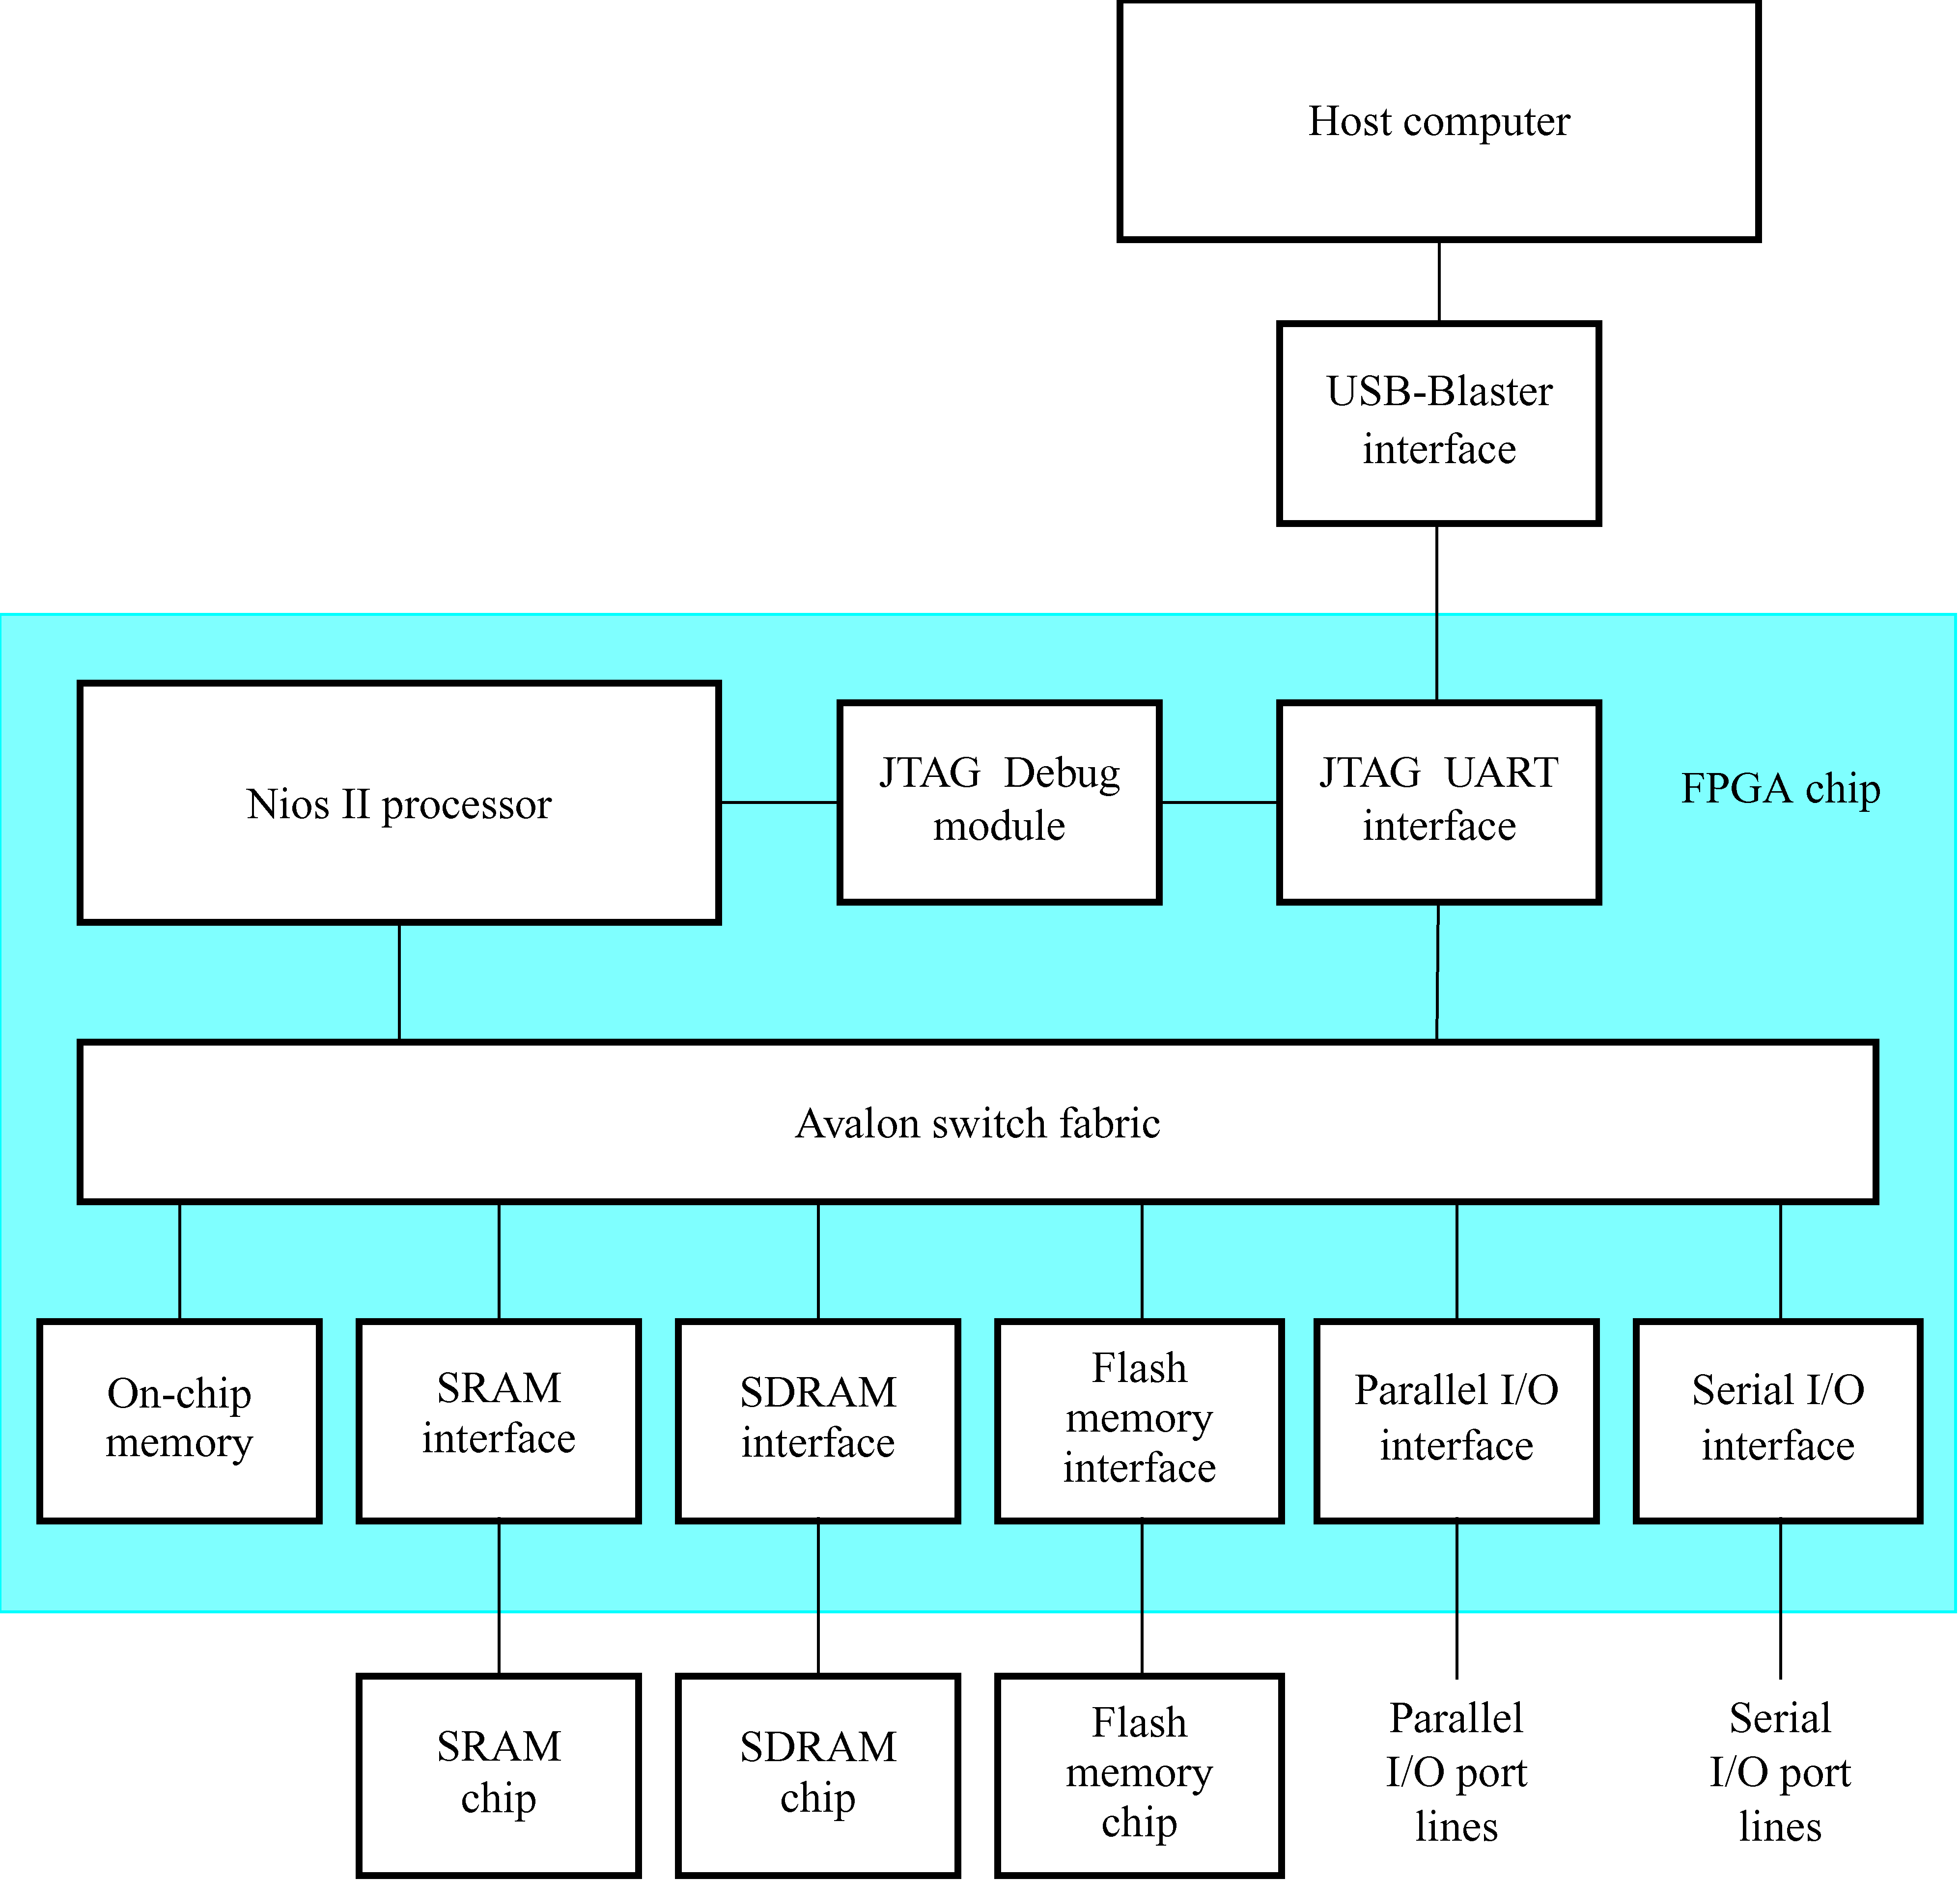
\includegraphics[scale=0.85]{figures/figure1.png}
   \caption{A Nios II system implemented on a DE-series board.} 
	 \label{fig:1}
	 \end{center}
\end{figure}

\newpage
The Nios II processor and the interfaces needed to connect to other chips on the
board are implemented in the FPGA chip. These components are
interconnected by means of the interconnection network called the Avalon\textsuperscript{\textregistered} Switch Fabric.
Memory blocks in the FPGA device can be used to provide an on-chip memory
for the Nios II processor. They can be connected to the processor either directly or
through the Avalon network. The SRAM and SDRAM memory chips on the board
are accessed through the appropriate interfaces. Input/output interfaces are
instantiated to provide connection to the I/O devices used in the system. 
A special JTAG* UART interface is used to connect to the circuitry that provides a 
Universal Serial Bus (USB) link to the host computer to which the DE-series board is connected. 
This circuitry and the associated software is called the {\it USB-Blaster}. 
Another module, called the JTAG Debug module, is provided to allow the host computer 
to control the Nios II processor.
It makes it possible to perform operations such as downloading programs into memory,
starting and stopping execution, setting program breakpoints, and collecting real-time
execution trace data.

Since all parts of the Nios II system implemented on the FPGA chip are defined by
using a hardware description language, a knowledgeable user could write such code
to implement any part of the system. This would be an onerous and time consuming
task. Instead, one can use the SOPC Builder or Platform Designer tools in the Quartus Prime software
to implement a desired system simply by
choosing the required components and specifying the parameters needed to make
each component fit the overall requirements of the system.

\section{Overview of Nios\textsuperscript{\textregistered} II Processor Features}
The Nios II processor has a number of features that can be configured
by the user to meet the demands of a desired system. The processor can be implemented
in three different configurations:
\begin{itemize}
\item Nios II/f is a "fast" version designed for superior performance.
It has the widest scope of configuration options that can be used to optimize
the processor for performance.
\item Nios II/s is a "standard" version that requires less resources in an FPGA
device as a trade-off for reduced performance.
\item Nios II/e is an "economy" version which requires the least amount of FPGA
resources, but also has the most limited set of user-configurable features.
\end{itemize}
 

The Nios II processor has a Reduced Instruction Set Computer (RISC) architecture.
Its arithmetic and logic operations are performed on operands in the general
purpose registers. The data is moved between the memory and these registers by
means of Load and Store instructions.

The wordlength of the Nios II processor is 32 bits. All registers are 32 bits long.
Byte addresses in a 32-bit word are assigned in {\it little-endian} style, 
in which the lower byte addresses are used for the
less significant bytes (the rightmost bytes) of the word. The Nios II architecture uses separate instruction and data buses, which is
often referred to as the {\it Harvard} architecture. 

A Nios II processor may operate in the following modes:
\begin{itemize}
\item {\it Supervisor mode} -- allows the processor to execute all instructions
and perform all available functions. When the processor is reset, it enters this mode.
\item {\it User mode} -- the intent of this mode is to prevent execution of some 
instructions that should be used for systems purposes only. This mode is available only
when the processor is configured  to use the Memory Management Unit (MMU) or the
Memory Protection Unit (MPU).
\end{itemize}
\noindent Application programs can be run in either the User or Supervisor modes.

\section{Register Structure}
The Nios II processor has thirty-two 32-bit general-purpose registers, 
as shown in Figure~\ref{fig:2}. Some of these registers are intended for a specific purpose
and have special names that are recognized by the Assembler.
\begin{itemize}
\item Register {\it r0} is referred to as the {\it zero} register. 
It always contains the constant 0.
Thus, reading this register returns the value 0, while writing to it has no effect.
\item Register {\it r1} is used by the Assembler as a temporary register; it should
not be referenced in user programs
\item Registers {\it r24} and {\it r29} are used for processing of exceptions;
they are not available in User mode
\item Registers {\it r25} and {\it r30} are used exclusively by the JTAG Debug module
\item Registers {\it r27} and {\it r28} are used to control the stack used by
the Nios II processor
\item Register {\it r31} is used to hold the return address when a subroutine is called
\end{itemize}

\begin{figure}[H]
\begin{center}
\begin{tabular}{|l|l|l|} \hline 
\rule{0in}{0.1in}{\bf Register} & {\bf Name} & {\bf Function} \\ \hline
r0 & zero & 0x00000000\\ 
r1 & at & Assembler Temporary\\ 
r2 & &\\ 
r3 & &\\ 
$\cdot$ & $\cdot$ & $\cdot$ \\ 
$\cdot$ & $\cdot$ & $\cdot$ \\ 
$\cdot$ & $\cdot$ & $\cdot$ \\ 
r23 & & \\
r24 & et & Exception Temporary {\it (1)} \\
r25 & bt & Breakpoint Temporary {\it (2)} \\
r26 & gp & Global Pointer \\
r27 & sp & Stack Pointer \\
r28 & fp & Frame Pointer \\
r29 & ea & Exception Return Address {\it (1)} \\ 
r30 & ba & Breakpoint Return Address {\it (2)} \\ 
r31 & ra & Return Address\\ \hline
\multicolumn{3}{|l|}{{\it (1)} The register is not available in User mode} \\
\multicolumn{3}{|l|}{{\it (2)} The register is used exclusively by the JTAG Debug module} \\ \hline
\end{tabular}
\end{center}
	\caption{General-purpose registers.}
	\label{fig:2}
\end{figure}

 

Nios II can have a number of 32-bit control registers. The number of registers depends on 
whether the MMU or the MPU features are implemented. 
There are six basic control registers, as indicated in Figure~\ref{fig:3}. The names given in
the figure are recognized by the Assembler. 
The registers are used as follows:
\begin{itemize}
\item Register {\it ctl0} reflects the operating status of the processor.
Two bits of this register are always used:
\begin{itemize}
\item $U$ is the User/Supervisor mode bit; 
$U = 1$ for User mode, while $U = 0$ for Supervisor mode. 
\item {\it PIE} is the processor interrupt-enable bit. When {\it PIE} = 1, the processor
may accept external interrupts. When {\it PIE} = 0, the processor ignores external interrupts.
\end{itemize}
\noindent
The rest of the bits (labeled as reserved in the figure) are used when MMU or MPU features
are implemented.
\item Register {\it ctl1} holds a saved copy of the status register during exception
processing. The bits {\it EU} and {\it EPIE} are the saved values of the
status bits $U$ and {\it PIE}.
\item Register {\it ctl2} holds a saved copy of the status register during debug break
processing. The bits {\it BU} and {\it BPIE} are the saved values of the
status bits $U$ and {\it PIE}.
\item Register {\it ctl3} is used to enable individual external interrupts. Each bit
corresponds to one of the interrupts {\it irq0} to {\it irq31}. The value of 1 means 
that the interrupt is enabled, while 0 means that it is disabled.
\item Register {\it ctl4} indicates which interrupts are pending. The value of a given
bit, $ctl4_k$, is set to 1 if the interrupt {\it irqk} is both active and enabled by
having the interrupt-enable bit, $ctl3_k$, set to 1.  
\item Register {\it ctl5} holds a value that uniquely identifies the processor in
a multiprocessor system.
\end{itemize}
 
\begin{figure}[H]
\begin{center}
\begin{tabular}{|l|l|lll|c|c|} \hline 
\rule{0in}{0.1in}{\bf Register} & {\bf Name} & $b_{31}$ & $\cdots$ & $b_2$ & $b_1$ & $b_0$ \\ \hline
ctl0 & status & \multicolumn{3}{|c|}{Reserved} & U & PIE \\ 
ctl1 & estatus & \multicolumn{3}{|c|}{Reserved} & EU & EPIE \\ 
ctl2 & bstatus & \multicolumn{3}{|c|}{Reserved} & BU & BPIE \\ \hline
ctl3 & ienable & \multicolumn{5}{|c|}{Interrupt-enable bits} \\
ctl4 & ipending & \multicolumn{5}{|c|}{Pending-interrupt bits} \\
ctl5 & cpuid & \multicolumn{5}{|c|}{Unique processor identifier} \\ \hline
\end{tabular}
\end{center}
	\caption{Basic control registers.}
	\label{fig:3}
\end{figure}

\noindent
The control registers can be read from and written to by special instructions
{\sf rdctl} and {\sf wrctl}, which can be executed only in the supervisor mode.

\section{Accessing Memory and I/O Devices}

Figure~\ref{fig:4} shows how a Nios II processor can access memory and I/O devices.
For best performance, the Nios II/f processor can include both instruction and 
data caches. The caches are implemented in the FPGA memory blocks. Their usage is
optional and they are specified (including their size) at the
system generation time by using the SOPC Builder or Platform Designer. The Nios II/s version can have
the instruction cache but not the data cache. The Nios II/e version has neither the
instruction nor data cache.

Another way to give the processor fast access to the on-chip memory is by using the 
{\it tightly coupled} memory arrangement, in which case the processor accesses the
memory via a direct path rather than through the Avalon network. Accesses to a tightly
coupled memory bypass the cache memory.
There can be one or more tightly coupled instruction and data memories.
If the instruction cache is not included in a system, then there must be at least
one tightly coupled memory provided for Nios II/f and Nios II/s processors.
On-chip memory can also be accessed via the Avalon network.

Off-chip memory devices, such as SRAM, SDRAM, and Flash memory chips are accessed
by instantiating the appropriate interfaces. The input/output devices are 
memory mapped and can be accessed as memory locations.

Data accesses to memory locations and I/O interfaces are performed by means of
Load and Store instructions, which cause data to be transferred between the memory 
and general-purpose registers.
 
\begin{figure}[H]
   \begin{center}
      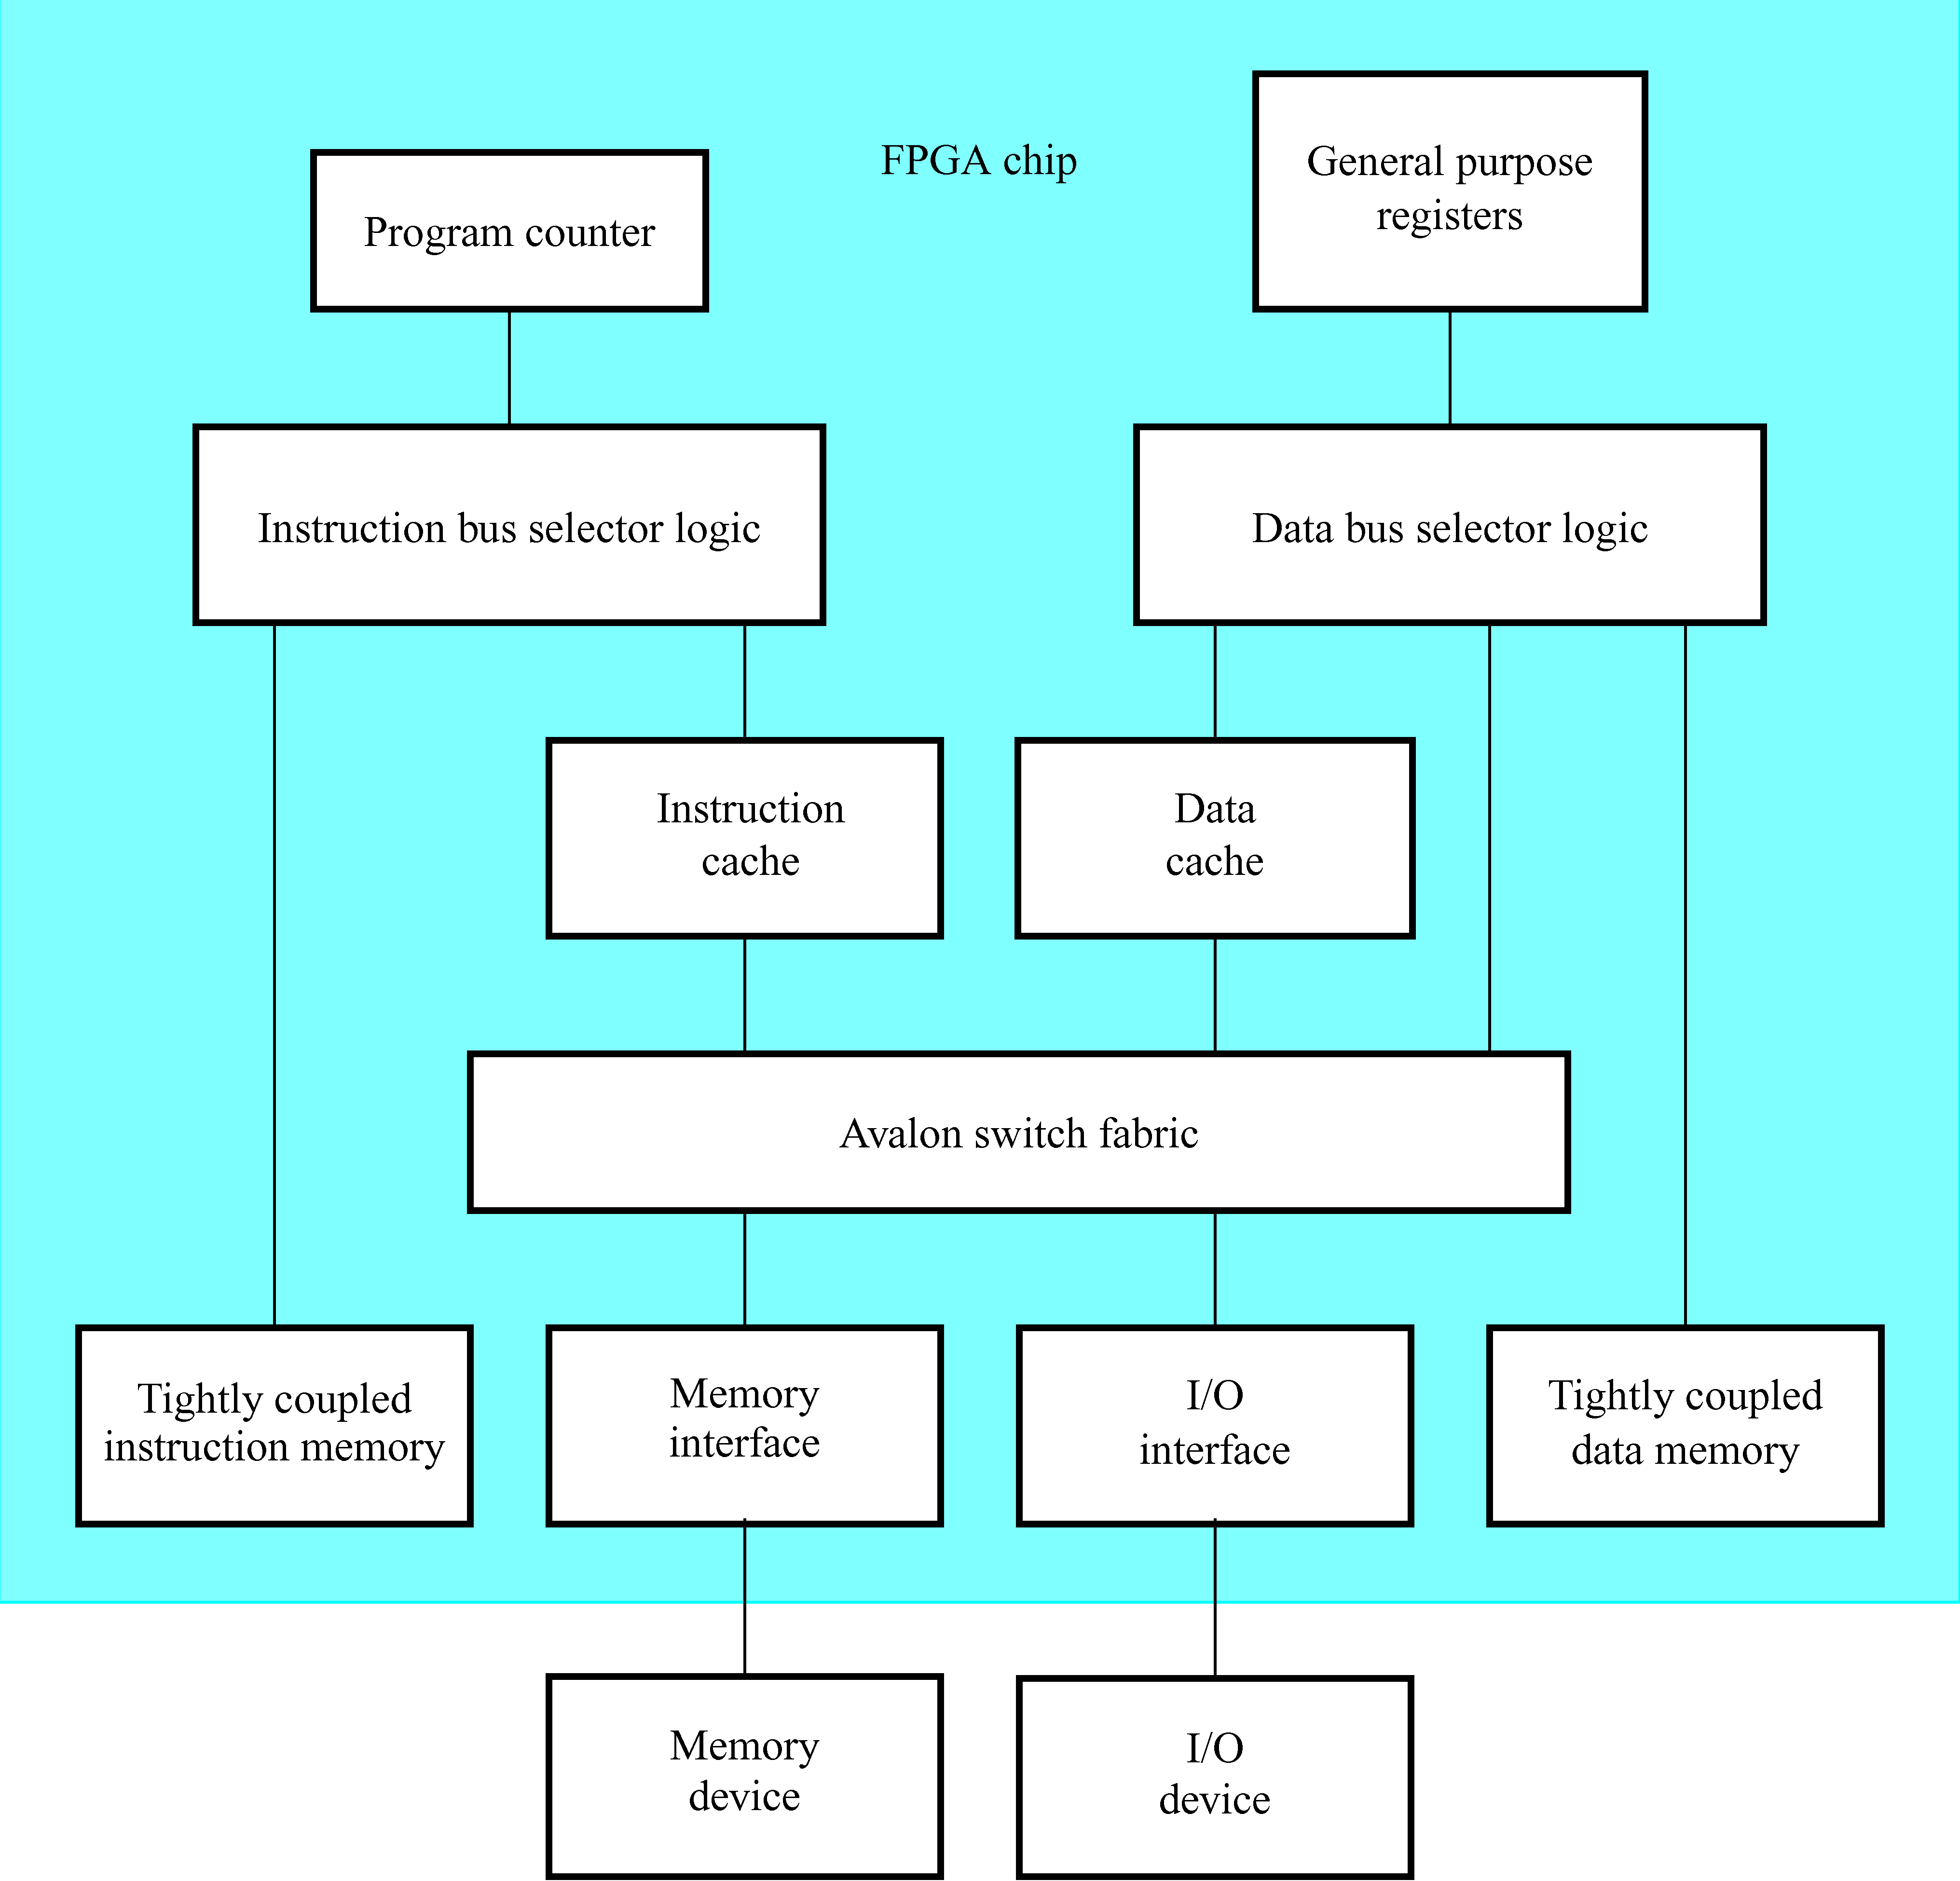
\includegraphics[scale=0.83]{figures/figure4.png}
   \caption{Memory and I/O organization.} 
	 \label{fig:4}
	 \end{center}
\end{figure}

\section{Addressing}
The Nios II processor issues 32-bit addresses. The memory space is byte-addressable.
Instructions can read and write {\it words} (32 bits), {\it halfwords} (16 bits),
or {\it bytes} (8 bits) of data. Reading or writing to an address that does not
correspond to an existing memory or I/O location produces an undefined result.

There are five addressing modes provided:
\begin{itemize}
\item {\it Immediate mode} -- a 16-bit operand is given explicitly in the instruction. 
This value may be sign extended to produce a 32-bit operand in instructions that perform 
arithmetic operations.
\item {\it Register mode} -- the operand is in a processor register
\item {\it Displacement mode} -- the effective address of the operand is the sum of the 
contents of a register and a signed 16-bit displacement value given in the instruction
\item {\it Register indirect mode} -- the effective address of the operand is the contents
of a register specified in the instruction. This is equivalent to the displacement mode
where the displacement value is equal to 0.
\item {\it Absolute mode} -- a 16-bit absolute address of an operand can be specified
by using the displacement mode with register {\it r0} which always contains the value 0.
\end{itemize}

\section{Instructions}

All Nios II instructions are 32-bits long. In addition to machine instructions that are
executed directly by the processor, the Nios II instruction set includes a number of
{\it pseudoinstructions} that can be used in assembly language programs. 
The Assembler replaces each pseudoinstruction by one or more machine instructions.

Figure~\ref{fig:5} depicts the three possible instruction formats: I-type, R-type and J-type.
In all cases the six bits $b_{5-0}$ denote the OP code. The remaining bits are used to
specify registers, immediate operands, or extended OP codes. 
\begin{itemize}
\item I-type -- Five-bit fields A and B are used to specify general-purpose registers.
A 16-bit field IMMED16 provides immediate data which can be sign extended to provide a
32-bit operand.
\item R-type -- Five-bit fields A, B and C are used to specify general-purpose registers.
An 11-bit field OPX is used to extend the OP code.
\item J-type -- A 26-bit field IMMED26 contains an unsigned immediate value. This format is
used only in the Call instruction.
\end{itemize}
 
\begin{figure}[H]
   \begin{center}
      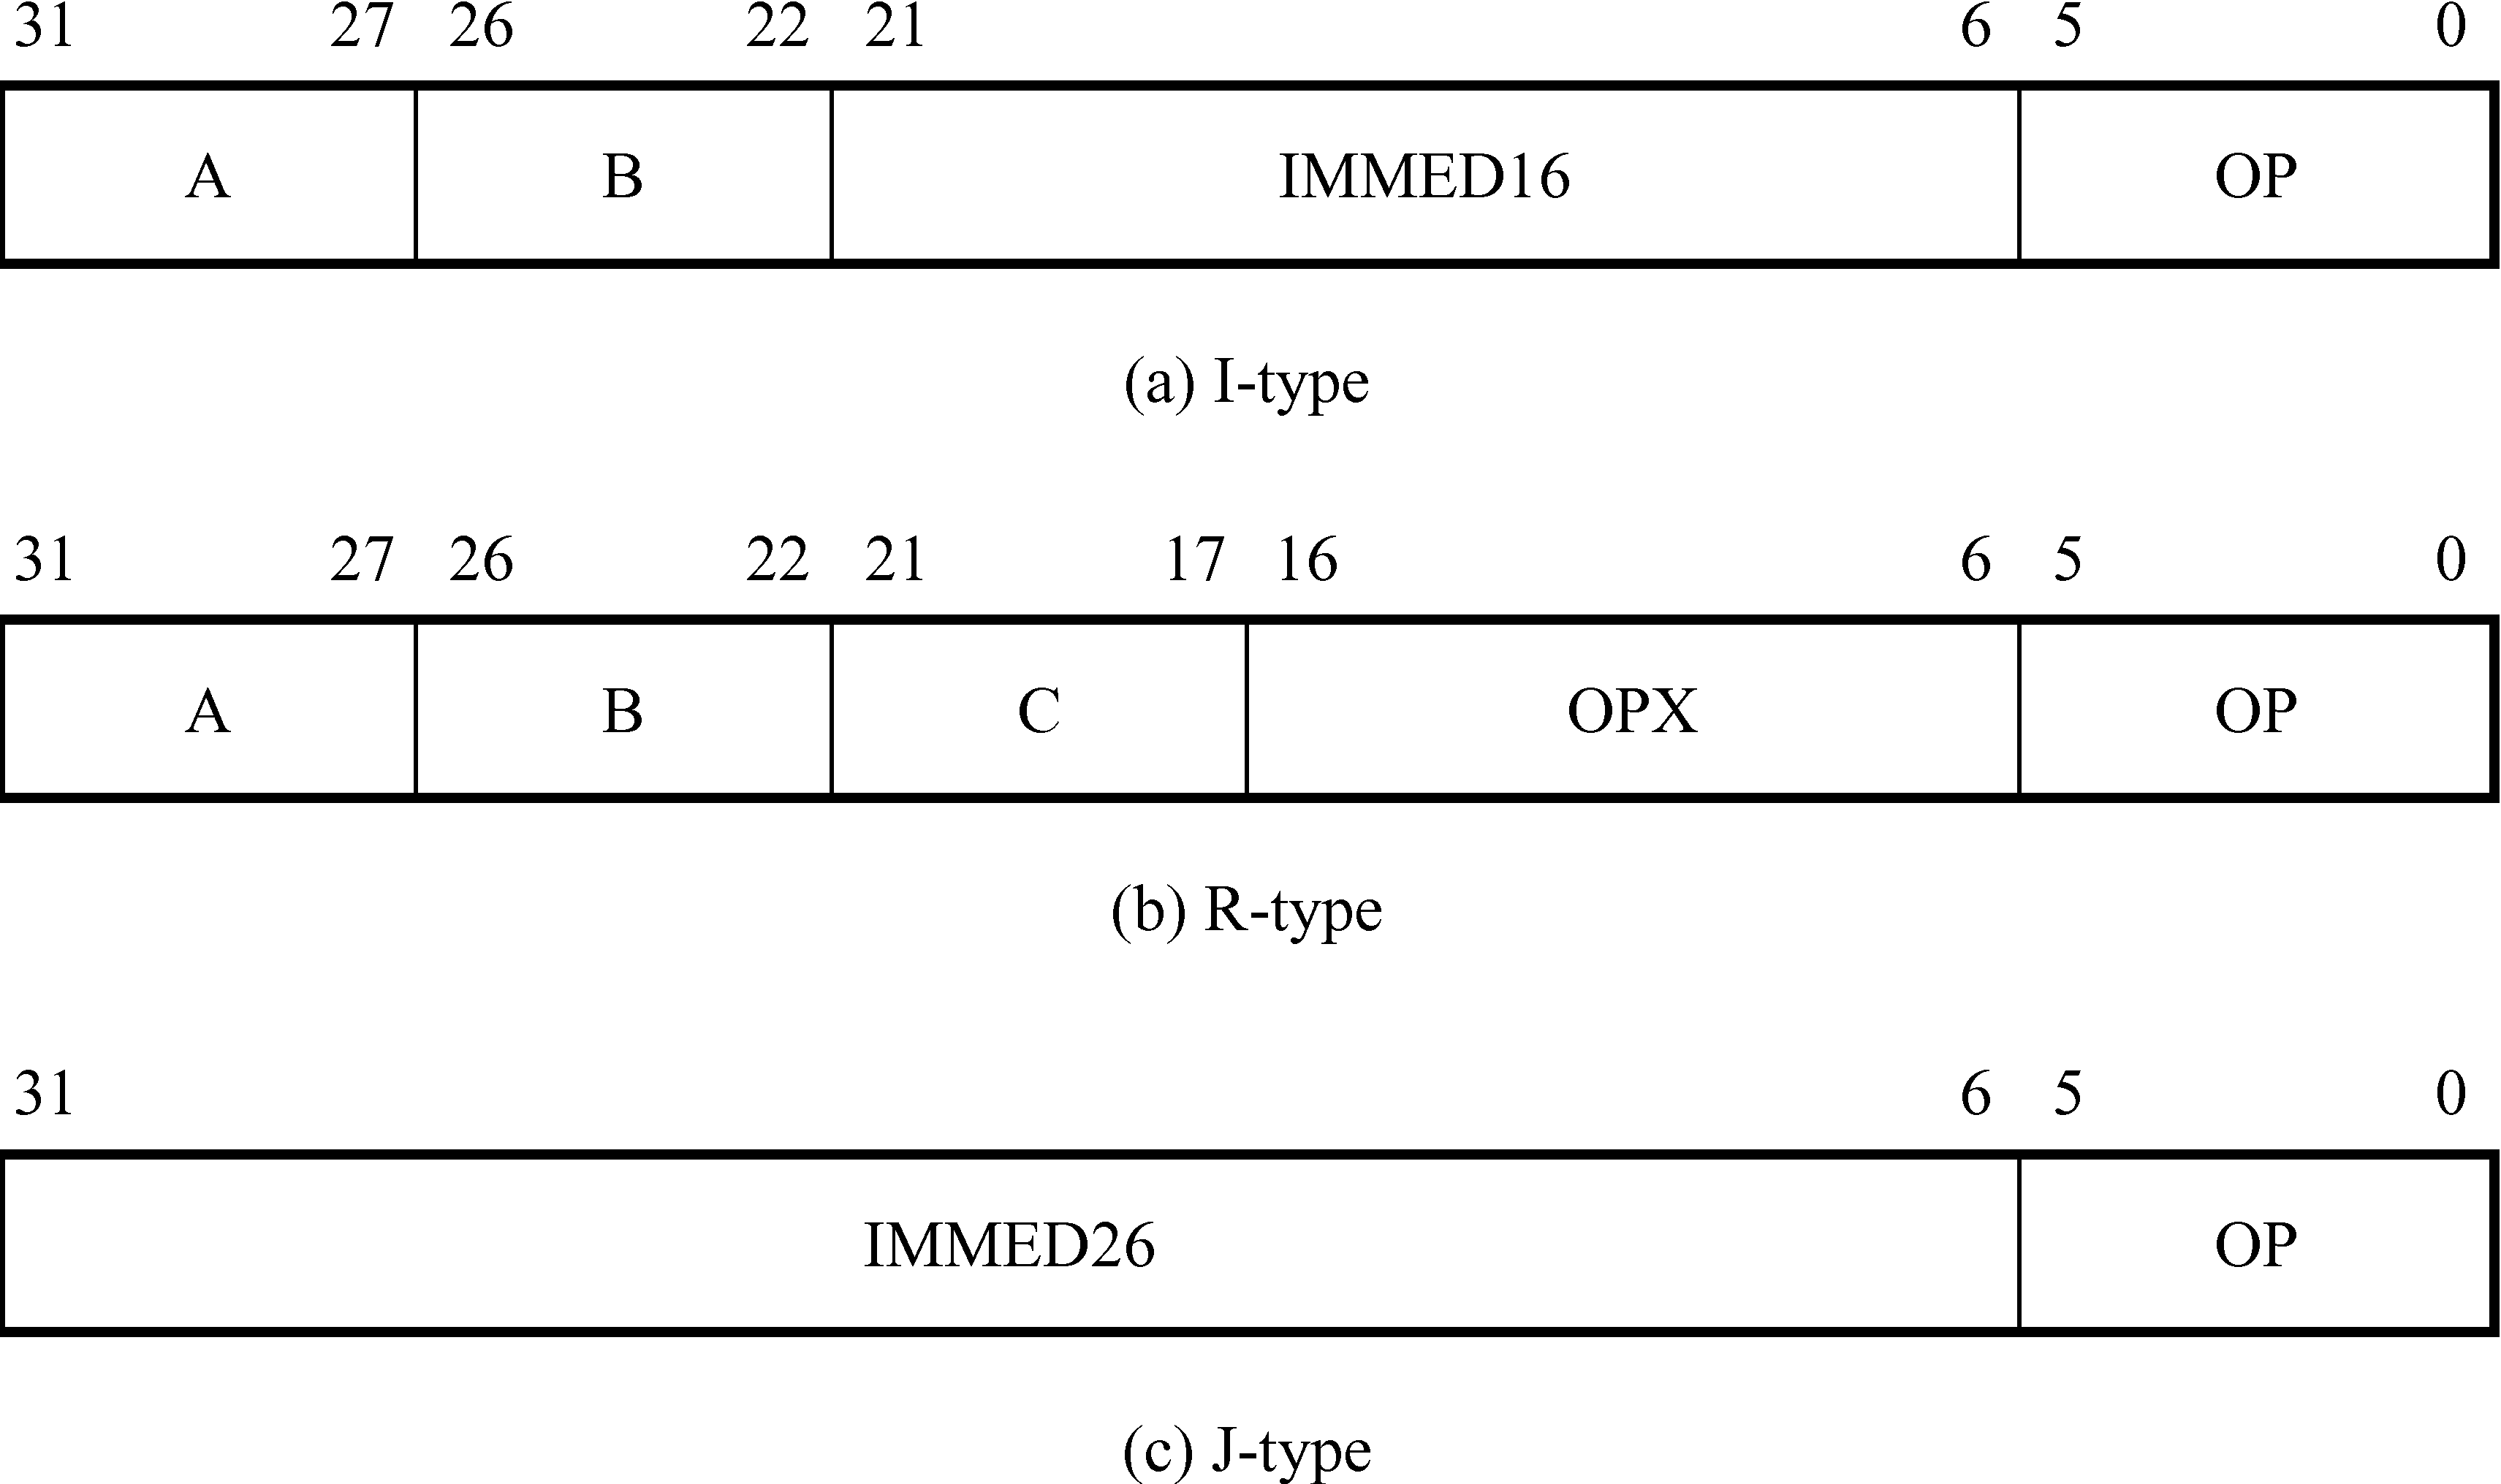
\includegraphics[scale=1]{figures/figure5.png}
   \caption{Formats of Nios II instructions.} 
	 \label{fig:5}
	 \end{center}
\end{figure}

The following subsections discuss briefly the main features of the Nios II instruction set.
For a complete description of the instruction set, including the details of how each
instruction is encoded, the reader should consult the {\it Nios II Processor Reference Handbook}.

\subsection{Load and Store Instructions}

Load and Store instructions are used to move data between memory (and I/0 interfaces)
and the general-purpose registers. They are of I-type. For example, the Load Word instruction
\begin{center}
{\sf ldw~~rB, byte\_offset(rA)}
\end{center}
\noindent
determines the effective address of a memory location as the sum of a byte\_offset value and 
the contents of register $A$. The 16-bit byte\_offset value is sign extended to 32 bits.
The 32-bit memory operand is loaded into register $B$.

For instance, assume that the contents of register $r4$ are $1260_{10}$ and the byte\_offset value is 
$80_{10}$. Then, the instruction
\begin{center}
{\sf ldw~~r3, 80(r4)}
\end{center}
\noindent
loads the 32-bit operand at memory address $1340_{10}$ into register $r3$. 
 

The Store Word instruction has the format
\begin{center}
{\sf stw~~rB, byte\_offset(rA)}
\end{center}
\noindent 
It stores the contents of register $B$ into the memory location at the address
computed as the sum of the byte\_offset value and the contents of register $A$. 
 
 
There are Load and Store instructions that use operands that are only 8 or 16 bits long.
They are referred to as Load/Store Byte and Load/Store Halfword instructions, respectively.
Such Load instructions are: 
\begin{itemize}
\item {\sf ldb} (Load Byte)
\item {\sf ldbu} (Load Byte Unsigned)
\item {\sf ldh} (Load Halfword)
\item {\sf ldhu} (Load Halfword Unsigned)
\end{itemize}
\noindent
When a shorter operand is loaded into a 32-bit register, its value has to be adjusted
to fit into the register. This is done by sign extending the 8- or 16-bit value to 32 bits
in the {\sf ldb} and {\sf ldh} instructions. In the {\sf ldbu} and {\sf ldhu} instructions
the operand is zero extended.
 

The corresponding Store instructions are: 
\begin{itemize}
\item {\sf stb} (Store Byte)
\item {\sf sth} (Store Halfword)
\end{itemize}
\noindent
The {\sf stb} instruction stores the low byte of register $B$ into the memory byte
specified by the effective address. The {\sf sth} instruction stores the low halfword
of register $B$. In this case the effective address must be halfword aligned.
 

Each Load and Store instruction has a version intended for accessing
locations in I/O device interfaces. These instructions are: 
\begin{itemize}
\item {\sf ldwio}~~~(Load Word I/O)
\item {\sf ldbio}~~~(Load Byte I/O)
\item {\sf ldbuio}~~~(Load Byte Unsigned I/O)
\item {\sf ldhio}~~~(Load Halfword I/O)
\item {\sf ldhuio}~~~(Load Halfword Unsigned I/O)
\item {\sf stwio}~~~(Store Word I/O)
\item {\sf stbio}~~~(Store Byte I/O)
\item {\sf sthio}~~~(Store Halfword I/O)
\end{itemize}
\noindent
The difference is that these instructions bypass the cache, if one exists.

\subsection{Arithmetic Instructions}

The arithmetic instructions operate on the data that is either in the general purpose registers or 
given as an immediate value in the instruction. These instructions are of R-type or I-type, respectively.
They include: 
\begin{itemize}
\item {\sf add} (Add Registers)
\item {\sf addi} (Add Immediate)
\item {\sf sub} (Subtract Registers)
\item {\sf subi} (Subtract Immediate)
\item {\sf mul} (Multiply)
\item {\sf muli} (Multiply Immediate)
\item {\sf div} (Divide)
\item {\sf divu} (Divide Unsigned)
\end{itemize}
\noindent
The Add instruction
\begin{center}
{\sf add~~rC, rA, rB}
\end{center}
\noindent
adds the contents of registers $A$ and $B$, and places the sum into register $C$.
 

\noindent
The Add Immediate instruction
\begin{center}
{\sf addi~~rB, rA, IMMED16}
\end{center}
\noindent
adds the contents of register $A$ and the sign-extended 16-bit operand given in the instruction,
and places the result into register $B$.
The addition operation in these instructions is the same for both signed and unsigned operands; 
there are no condition flags that are set by the operation. 
This means that when unsigned operands are added, the carry from
the most significant bit position has to be detected by executing a separate instruction.
Similarly, when signed operands are added, the arithmetic overflow has to be detected separately.
The detection of these conditions is discussed in section 8.11.
 

\noindent
The Subtract instruction
\begin{center}
{\sf sub~~rC, rA, rB}
\end{center}
\noindent
subtracts the contents of register $B$ from register $A$, and places the result into register $C$.
Again, the carry and overflow detection has to be done by using additional instructions,
as explained in section 8.11.
 

\noindent
The immediate version, {\sf subi}, is a pseudoinstruction implemented as
\begin{center}
{\sf addi~~rB, rA, -IMMED16}
\end{center}
 

\noindent
The Multiply instruction
\begin{center}
{\sf mul~~rC, rA, rB}
\end{center}
\noindent
multiplies the contents of registers $A$ and $B$, and places the low-order 32 bits of the product
into register $C$. The operands are treated as unsigned numbers. The carry and overflow
detection has to be done by using additional instructions. In the immediate version
\begin{center}
{\sf muli~~rB, rA, IMMED16}
\end{center}
\noindent
the 16-bit immediate operand is sign extended to 32 bits.
 
\noindent
The Divide instruction
\begin{center}
{\sf div~~rC, rA, rB}
\end{center}
\noindent
divides the contents of register $A$ by the contents of register $B$ and places the integer
portion of the quotient into register $C$. The operands are treated as signed integers.
The {\sf divu} instruction is performed in the same way except that the operands are treated 
as unsigned integers.

\subsection{Logic Instructions}

The logic instructions provide the AND, OR, XOR, and NOR operations. They operate on data
that is either in the general purpose registers or given as an immediate value in the instruction. 
These instructions are of R-type or I-type, respectively.
 

\noindent
The AND instruction
\begin{center}
{\sf and~~rC, rA, rB} 
\end{center}
\noindent
performs a bitwise logical AND of the contents of registers $A$ and $B$, and stores the result
in register $C$. Similarly, the instructions {\sf or}, {\sf xor} and {\sf nor} perform the OR, XOR 
and NOR operations, respectively.
 

\noindent
The AND Immediate instruction
\begin{center}
{\sf andi~~rB, rA, IMMED16} 
\end{center}
\noindent
performs a bitwise logical AND of the contents of register $A$ and the IMMED16 operand
which is zero-extended to 32 bits, and stores the result in register $B$.
Similarly, the instructions {\sf ori}, {\sf xori} and {\sf nori} perform the OR, XOR 
and NOR operations, respectively.
 
 
\noindent
It is also possible to use the 16-bit immediate
operand as the 16 high-order bits in the logic operations, in which case the low-order 16 bits 
of the operand are zeros. This is accomplished with the instructions: 
\begin{itemize}
\item {\sf andhi}~~~(AND High Immediate) 
\item {\sf orhi}~~~(OR High Immediate)
\item {\sf xorhi}~~~(XOR High Immediate)
\end{itemize}

\subsection{Move Instructions}

The Move instructions copy the contents of one register into another, or they place an immediate
value into a register. They are pseudoinstructions implemented by using other instructions.
The instruction
\begin{center}
{\sf mov~~rC, rA}
\end{center}
\noindent
copies the contents of register $A$ into register $C$. It is implemented as 
\begin{center}
{\sf add~~rC, rA, r0}
\end{center}
 

\noindent
The Move Immediate instruction
\begin{center}
{\sf movi~~rB, IMMED16}
\end{center}
\noindent
sign extends the IMMED16 value to 32 bits and loads it into register $B$.
It is implemented as
\begin{center}
{\sf addi~~rB, r0, IMMED16}
\end{center}
 

\noindent
The Move Unsigned Immediate instruction
\begin{center}
{\sf movui~~rB, IMMED16}
\end{center}
\noindent
zero extends the IMMED16 value to 32 bits and loads it into register $B$.
It is implemented as
\begin{center}
{\sf ori~~rB, r0, IMMED16}
\end{center}
 

\noindent
The Move Immediate Address instruction
\begin{center}
{\sf movia~~rB, LABEL}
\end{center}
\noindent
loads a 32-bit value that corresponds to the address {\it LABEL} into register $B$.
It is implemented as:
\begin{center}
\begin{tabular}{ll}
{\sf orhi} & {\sf rB, r0, \%hi(LABEL)} \\
{\sf ori} & {\sf rB, rB, \%lo(LABEL)}
\end{tabular}
\end{center} 
\noindent
The {\sf \%hi(LABEL)} and {\sf \%lo(LABEL)} are the Assembler macros which extract the
high-order 16 bits and the low-order 16 bits, respectively, of a 32-bit value {\it LABEL}.
The {\sf orhi} instruction sets the high-order bits of register $B$, followed
by the {\sf ori} instruction which sets the low-order bits of $B$. Note that 
two instructions are used because the I-type format provides for only a 16-bit
immediate operand.

\subsection{Comparison Instructions}

The Comparison instructions compare the contents of two registers or the contents of a
register and an immediate value, and write either 1 (if true) or 0 (if false) into 
the result register. They are of R-type or I-type, respectively. 
These instructions correspond to the equality and relational operators in the
C programming language. 
 

\noindent
The Compare Less Than Signed instruction
\begin{center}
{\sf cmplt~~rC, rA, rB}
\end{center}
\noindent
performs the comparison of signed numbers in registers $A$ and $B$, {\sf rA $<$ rB}, and writes 
a 1 into register $C$ if the result is true; otherwise, it writes a 0.
 

\noindent
The Compare Less Than Unsigned instruction
\begin{center}
{\sf cmpltu~~rC, rA, rB}
\end{center}
\noindent
performs the same function as the {\sf cmplt} instruction, but it treats the operands as
unsigned numbers.
 

\noindent
Other instructions of this type are:
\begin{itemize}
\item {\sf cmpeq~~rC, rA, rB}~~~(Comparison rA == rB)
\item {\sf cmpne~~rC, rA, rB}~~~(Comparison rA != rB)
\item {\sf cmpge~~rC, rA, rB}~~~(Signed comparison rA $>$= rB)
\item {\sf cmpgeu~~rC, rA, rB}~~~(Unsigned comparison rA $>$= rB)
\item {\sf cmpgt~~rC, rA, rB}~~~(Signed comparison rA $>$ rB) \\
This is a pseudoinstruction implemented as the {\sf cmplt} instruction by swapping
its rA and rB operands.
\item {\sf cmpgtu~~rC, rA, rB}~~~(Unsigned comparison rA $>$ rB) \\
This is a pseudoinstruction implemented as the {\sf cmpltu} instruction by swapping
its rA and rB operands.
\item {\sf cmple~~rC, rA, rB}~~~(Signed comparison rA $<$= rB) \\
This is a pseudoinstruction implemented as the {\sf cmpge} instruction by swapping
its rA and rB operands.
\item {\sf cmpleu~~rC, rA, rB}~~~(Unsigned comparison rA $<$= rB) \\
This is a pseudoinstruction implemented as the {\sf cmpgeu} instruction by swapping
its rA and rB operands.
\end{itemize}

The immediate versions of the Comparison instructions involve an immediate operand.
For example, the Compare Less Than Signed Immediate instruction
\begin{center}
{\sf cmplti~~rB, rA, IMMED16}
\end{center}
\noindent
compares the signed number in register $A$ with the sign-extended immediate operand. 
It writes a 1 into register $B$ if {\sf rA $<$ IMMED16}; 
otherwise, it writes a 0.
 

\noindent
The Compare Less Than Unsigned Immediate instruction
\begin{center}
{\sf cmpltui~~rB, rA, IMMED16}
\end{center}
\noindent
compares the unsigned number in register $A$ with the zero-extended immediate operand. 
It writes a 1 into register $B$ if {\sf rA $<$ IMMED16}; 
otherwise, it writes a 0.
 

\noindent
Other instructions of this type are:
\begin{itemize}
\item {\sf cmpeqi~~rB, rA, IMMED16}~~~(Comparison rA == IMMED16)
\item {\sf cmpnei~~rB, rA, IMMED16}~~~(Comparison rA != IMMED16)
\item {\sf cmpgei~~rB, rA, IMMED16}~~~(Signed comparison rA $>$= IMMED16)
\item {\sf cmpgeui~~rB, rA, IMMED16}~~~(Unsigned comparison rA $>$= IMMED16)
\item {\sf cmpgti~~rB, rA, IMMED16}~~~(Signed comparison rA $>$ IMMED16) \\
This is a pseudoinstruction which is implemented by using the {\sf cmpgei} instruction 
with an immediate value IMMED16 + 1.
\item {\sf cmpgtui~~rB, rA, IMMED16}~~~(Unsigned comparison rA $>$ IMMED16) \\
This is a pseudoinstruction which is implemented by using the {\sf cmpgeui} instruction 
with an immediate value IMMED16 + 1.
\item {\sf cmplei~~rB, rA, IMMED16}~~~(Signed comparison rA $<$= IMMED16) \\
This is a pseudoinstruction which is implemented by using the {\sf cmplti} instruction with
an immediate value IMMED16 + 1.
\item {\sf cmpleui~~rB, rA, IMMED16}~~~(Unsigned comparison rA $<$= IMMED16) \\
This is a pseudoinstruction which is implemented by using the {\sf cmpltui} instruction with
an immediate value IMMED16 + 1.
\end{itemize}

\subsection{Shift Instructions}

The Shift instructions shift the contents of a register either to the right or to the left.
They are of R-type. They correspond to the shift operators, $>$> and $<$<, in the C programming
language. These instructions are:
\begin{itemize}
\item {\sf srl~~rC, rA, rB}~~~(Shift Right Logical)
\item {\sf srli~~rC, rA, IMMED5}~~~(Shift Right Logical Immediate)
\item {\sf sra~~rC, rA, rB}~~~(Shift Right Arithmetic)
\item {\sf srai~~rC, rA, IMMED5}~~~(Shift Right Arithmetic Immediate)
\item {\sf sll~~rC, rA, rB}~~~(Shift Left Logical)
\item {\sf slli~~rC, rA, IMMED5}~~~(Shift Left Logical Immediate)
\end{itemize}
\noindent
The {\sf srl} instruction shifts the contents of register $A$ to the right by the number 
of bit positions specified by the five least-significant bits (number in the range 0 to 31)
in register $B$, and stores the result in register $C$. The vacated bits on the left side
of the shifted operand are filled with 0s.
 

\noindent
The {\sf srli} instruction shifts the contents of register $A$ to the right by the number 
of bit positions specified by the five-bit unsigned value, IMMED5, given in the instruction.
 

\noindent
The {\sf sra} and {\sf srai} instructions perform the same actions as the {\sf srl} and 
{\sf srli} instructions, except that the sign bit, $rA_{31}$, is replicated into the vacated 
bits on the left side of the shifted operand.
 

\noindent
The {\sf sll} and {\sf slli} instructions are similar to the {\sf srl} and {\sf srli}
instructions, but they shift the operand in register $A$ to the left and fill the vacated
bits on the right side with 0s.

\subsection{Rotate Instructions}

There are three Rotate instructions, which use the R-type format:
\begin{itemize}
\item {\sf ror~~rC, rA, rB}~~~(Rotate Right)
\item {\sf rol~~rC, rA, rB}~~~(Rotate Left)
\item {\sf roli~~rC, rA, IMMED5}~~~(Rotate Left Immediate)
\end{itemize}
\noindent
The {\sf ror} instruction rotates the bits of register $A$ in the left-to-right direction
by the number of bit positions specified by the five least-significant bits 
(number in the range 0 to 31) in register $B$, and stores the result in register $C$.
 

\noindent
The {\sf rol} instruction is similar to the {\sf ror} instruction, but it rotates the 
operand in the right-to-left direction.
 

\noindent
The {\sf roli} instruction rotates the bits of register $A$ in the right-to-left
direction by the number of bit positions specified by the five-bit unsigned value, 
IMMED5, given in the instruction, and stores the result in register $C$.

\subsection{Branch and Jump Instructions}

The flow of execution of a program can be changed by executing Branch or Jump instructions.
It may be changed either unconditionally or conditionally.
 

\noindent
The Jump instruction
\begin{center}
{\sf jmp~~rA}
\end{center}
\noindent
transfers execution unconditionally to the address contained in register $A$.
 

\noindent
The Unconditional Branch instruction
\begin{center}
{\sf br~~LABEL}
\end{center}
\noindent
transfers execution unconditionally to the instruction at address {\it LABEL}.
This is an instruction of I-type, in which a 16-bit immediate value (interpreted as
a signed number) specifies the offset to the branch target instruction.
The offset is the distance in bytes from the instruction that immediately follows
{\sf br} to the address {\it LABEL}.
 

Conditional transfer of execution is achieved with the Conditional Branch instructions,
which compare the contents of two registers and cause a branch if the result is true.
These instructions are of I-type and the offset is determined as explained above for the 
{\sf br} instruction.

\noindent
The Branch if Less Than Signed instruction
\begin{center}
{\sf blt~~rA, rB, LABEL}
\end{center}
\noindent
performs the comparison ~{\sf rA $<$ rB}, treating the contents of the registers as signed numbers.
 

\noindent
The Branch if Less Than Unsigned instruction
\begin{center}
{\sf bltu~~rA, rB, LABEL}
\end{center}
\noindent
performs the comparison ~{\sf rA $<$ rB}, treating the contents of the registers as unsigned numbers.
 

\noindent
The other Conditional Branch instructions are:
\begin{itemize}
\item {\sf beq~~rA, rB, LABEL}~~~(Comparison rA == rB)
\item {\sf bne~~rA, rB, LABEL}~~~(Comparison rA != rB)
\item {\sf bge~~rA, rB, LABEL}~~~(Signed comparison rA $>$= rB)
\item {\sf bgeu~~rA, rB, LABEL}~~~(Unsigned comparison rA $>$= rB)
\item {\sf bgt~~rA, rB, LABEL}~~~(Signed comparison rA $>$ rB) \\
This is a pseudoinstruction implemented as the {\sf blt} instruction by swapping
the register operands.
\item {\sf bgtu~~rA, rB, LABEL}~~~(Unsigned comparison rA $>$ rB) \\
This is a pseudoinstruction implemented as the {\sf bltu} instruction by swapping
the register operands.
\item {\sf ble~~rA, rB, LABEL}~~~(Signed comparison rA $<$= rB) \\
This is a pseudoinstruction implemented as the {\sf bge} instruction by swapping
the register operands.
\item {\sf bleu~~rA, rB, LABEL}~~~(Unsigned comparison rA $<$= rB) \\
This is a pseudoinstruction implemented as the {\sf bgeu} instruction by swapping
the register operands.
\end{itemize}

\subsection{Subroutine Linkage Instructions}

Nios II has two instructions for calling subroutines. The Call Subroutine instruction
\begin{center}
{\sf call~~LABEL}
\end{center}
\noindent
is of J-type, which includes a 26-bit unsigned immediate value (IMMED26). 
The instruction saves the return address (which is the address of the next instruction) 
in register $r31$. Then, it transfers control to the instruction at address {\it LABEL}. 
This address is determined by concatenating the four high-order bits of the Program Counter 
with the IMMED26 value as follows
$$
{\rm Jump~address} = {\rm PC}_{31-28} : {\rm IMMED26} : 00
$$
\noindent
Note that the two least-significant bits are 0 because Nios II instructions must
be aligned on word boundaries.
 

\noindent
The Call Subroutine in Register instruction
\begin{center}
{\sf callr~~rA}
\end{center}
\noindent
is of R-type. It saves the return address in register $r31$ and then transfers control to the 
instruction at the address contained in register $A$.
 

Return from a subroutine is performed with the instruction
\begin{center}
{\sf ret}
\end{center}
\noindent
This instruction transfers execution to the address contained in register $r31$.

\subsection{Control Instructions}

The Nios II control registers can be read and written by special instructions.
The Read Control Register instruction
\begin{center}
{\sf rdctl~~rC, ctlN}
\end{center}
\noindent
copies the contents of control register {\it ctlN} into register $C$. 
 

\noindent
The Write Control Register instruction
\begin{center}
{\sf wrctl~~ctlN, rA}
\end{center}
\noindent
copies the contents of register A into the control register {\it ctlN}.
 

There are two instructions provided for dealing with exceptions: {\sf trap} and {\sf eret}.
They are similar to the {\sf call} and {\sf ret} instructions, but they are used for exceptions.
Their use is discussed in section 11.
 

The instructions {\sf break} and {\sf bret} generate breaks and return from breaks. They are used
exclusively by the software debugging tools.
 

The Nios II cache memories are managed with the instructions: {\sf flushd} (Flush Data Cache Line),
{\sf flushi} (Flush Instruction Cache Line), {\sf initd} (Initialize Data Cache Line), and
{\sf initi} (Initialize Instruction Cache Line). These instructions are discussed in section 12.1.

\subsection{Carry and Overflow Detection}

As pointed out in section 8.2, the Add and Subtract instructions perform the corresponding operations
in the same way for both signed and unsigned operands. The possible carry and arithmetic overflow
conditions are not detected, because Nios II does not contain condition flags that might be set as
a result. These conditions can be detected by using additional instructions.
 

Consider the Add instruction
\begin{center}
{\sf add~~rC, rA, rB}
\end{center}
\noindent
Having executed this instruction, a possible occurrence of a carry out of the most-significant
bit ($C_{31}$) can be detected by checking whether the unsigned sum (in register $C$) is less than
one of the unsigned operands. For example, if this instruction is followed by the instruction
\begin{center}
{\sf cmpltu~~rD, rC, rA}
\end{center}
\noindent
then the carry bit will be written into register $D$.
 

\noindent
Similarly, if a branch is required when a carry occurs, this can be accomplished as follows:
\begin{center}
\begin{tabular}{ll}
{\sf add} & {\sf rC, rA, rB} \\
{\sf bltu} & {\sf rC, rA, LABEL}
\end{tabular}
\end{center}
 

A test for arithmetic overflow can be done by checking the signs of the summands and the resulting
sum. An overflow occurs if two positive numbers produce a negative sum, or if two negative numbers
produce a positive sum. Using this approach, the overflow condition can control a conditional
branch as follows:
\begin{center}
\begin{tabular}{lll}
{\sf add} & {\sf rC, rA, rB}~~~~~~~ & /* The required Add operation */ \\
{\sf xor} & {\sf rD, rC, rA}  & /* Compare signs of sum and rA */ \\
{\sf xor} & {\sf rE, rC, rB}  & /* Compare signs of sum and rB */ \\
{\sf and} & {\sf rD, rD, rE}  & /* Set $D_{31} = 1$ if ($(A_{31} == B_{31})~!=~C_{31}$) */ \\
{\sf blt} & {\sf rD, r0, LABEL} & /* Branch if overflow occurred */
\end{tabular}
\end{center}
 

A similar approach can be used to detect the carry and overflow conditions in Subtract operations.
A carry out of the most-significant bit of the resulting difference can be detected by checking 
whether the first operand is less than the second operand. Thus, the carry can be used to control 
a conditional branch as follows:
\begin{center}
\begin{tabular}{ll}
{\sf sub} & {\sf rC, rA, rB} \\
{\sf bltu} & {\sf rA, rB, LABEL}
\end{tabular}
\end{center}

\noindent
The arithmetic overflow in a Subtract operation is detected by comparing the sign of the generated 
difference with the signs of the operands. Overflow occurs if the operands in registers $A$ and $B$ 
have different signs, and the sign of the difference in register $C$ is different than the sign of $A$.
Thus, a conditional branch based on the arithmetic overflow can be achieved as follows:
\begin{center}
\begin{tabular}{lll}
{\sf sub} & {\sf rC, rA, rB}~~~~~~~ & /* The required Subtract operation */ \\
{\sf xor} & {\sf rD, rA, rB}  & /* Compare signs of rA and rB */ \\
{\sf xor} & {\sf rE, rA, rC}  & /* Compare signs of rA and rC */ \\
{\sf and} & {\sf rD, rD, rE}  & /* Set $D_{31} = 1$ if $((A_{31}~!=~B_{31})~\&\&~(A_{31}~!=~C_{31})$) */ \\
{\sf blt} & {\sf rD, r0, LABEL} & /* Branch if overflow occurred */
\end{tabular}
\end{center}
 

\section{Assembler Directives}

The Nios II Assembler conforms to the widely used GNU* Assembler, which is 
software available in the public domain. Thus, the GNU Assembler directives can
be used in Nios II programs. Assembler directives begin with a period. 
We describe some of the more frequently used assembler directives below.
 

\noindent
{\sf .ascii}~~"{\it string}"...
 

\noindent
A string of ASCII characters is loaded into consecutive byte addresses in the memory.
Multiple strings, separated by commas, can be specified.
 

\noindent
{\sf .asciz}~~"{\it string}"...
 

\noindent
This directive is the same as {\sf .ascii}, except that each string is followed 
(terminated) by a zero byte.
 

\noindent
{\sf .byte}~~{\it expressions}
 

\noindent
Expressions separated by commas are specified. Each expression is assembled into
the next byte. Examples of expressions are: 8, 5 + LABEL, and K $-$ 6.
 
\newpage
\noindent
{\sf .data}
 

\noindent
Identifies the data that should be placed in the data section of the memory.
The desired memory location for the data section can be specified in the
\productNameMed{}'s system configuration window.
 

\noindent
{\sf .end}
 

\noindent
Marks the end of the source code file; everything after this
directive is ignored by the assembler.
 

\noindent
{\sf .equ}~~{\it symbol,~expression}
 

\noindent
Sets the value of {\it symbol} to {\it expression}.
 
\noindent
{\sf .global}~~{\it symbol}
 

\noindent
Makes {\it symbol} visible outside the assembled object file.
 

\noindent
{\sf .hword}~~{\it expressions}
 

\noindent
Expressions separated by commas are specified. Each expression is assembled into
a 16-bit number.
 

\noindent
{\sf .include}~~"{\it filename}"
 

\noindent
Provides a mechanism for including supporting files in a source program.
 

\noindent
{\sf .org}~~{\it new-lc}
 

\noindent
Advances the location counter by {\it new-lc}, where {\it new-lc} is used as
an offset from the starting location specified in the \productNameMed{}'s 
system configuration window. The {\sf .org} directive may only
increase the location counter, or leave it unchanged; it cannot move the
location counter backwards.
 

\noindent
{\sf .skip}~~{\it size}
 

\noindent
Emits the number of bytes specified in {\it size}; the value of each byte is zero.
 

\noindent
{\sf .text}
 

\noindent
Identifies the code that should be placed in the text section of the memory.
The desired memory location for the text section can be specified in the 
\productNameMed{}'s system configuration window.
 

\noindent
{\sf .word}~~{\it expressions}
 

\noindent
Expressions separated by commas are specified. Each expression is assembled into
a 32-bit number.
 
 

\section{Example Program}

As an illustration of Nios II instructions and assembler directives, 
Figure~\ref{fig:6} gives an assembly language program
that computes a dot product of two vectors, {\it A} and {\it B}. The vectors
have $n$ elements. The required computation is
\begin{center}
Dot product $=$ $\sum_{i = 0}^{n - 1}$ A({\it i}) $\times$ B({\it i})
\end{center}

\noindent
The vectors are stored in memory locations at addresses
{\it AVECTOR} and {\it BVECTOR}, respectively. The number of
elements, $n$, is stored in memory location $N$. The computed result is written
into memory location {\it DOT\_PRODUCT}. Each vector element is assumed to be a
signed 32-bit number.

\begin{figure}[H]
\begin{lstlisting}[style=defaultNiosStyle]
.include "nios_macros.s"
.global _start
_start:
        movia r2, AVECTOR         /* Register r2 is a pointer to vector A */
        movia r3, BVECTOR         /* Register r3 is a pointer to vector B */
        movia r4, N
        ldw   r4, 0(r4)           /* Register r4 is used as the counter for loop */
                                  /* iterations */
        add   r5, r0, r0          /* Register r5 is used to accumulate the */
                                  /* product */
LOOP:   ldw   r6, 0(r2)           /* Load the next element of vector A */
        ldw   r7, 0(r3)           /* Load the next element of vector B */
        mul   r8, r6, r7          /* Compute the product of next pair of elements */
        add   r5, r5, r8          /* Add to the sum */
        addi  r2, r2, 4           /* Increment the pointer to vector A */
        addi  r3, r3, 4           /* Increment the pointer to vector B */
        subi  r4, r4, 1           /* Decrement the counter */
        bgt   r4, r0, LOOP        /* Loop again if not finished */
        stw   r5, DOT_PRODUCT(r0) /* Store the result in memory */
STOP:   br    STOP
N:
.word 6                           /* Specify the number of elements */
AVECTOR:
.word 5, 3, -6, 19, 8, 12         /* Specify the elements of vector A */
BVECTOR:
.word 2, 14, -3, 2, -5, 36        /* Specify the elements of vector B */
DOT_PRODUCT:
.skip 4
\end{lstlisting}
	\caption{A program that computes the dot product of two vectors.}
	\label{fig:6}
\end{figure}
 

\noindent
Note that the program ends by continuously
looping on the last Branch instruction. If instead we wanted to pass control to
debugging software, we could replace this {\sf br} instruction with the {\sf break}
instruction.
  

The program includes the assembler directive
\begin{center}
{\sf .include~~"nios\_macros.s"}
\end{center}
\noindent
which informs the Assembler to use some macro commands that have been created
for the Nios II processor. In this program, the macro used
converts the {\sf movia} pseudoinstruction into two OR instructions as
explained in section 8.4.
 

The directive
\begin{center}
{\sf .global~~\_start}
\end{center} 
\noindent
indicates to the Assembler that the label {\it \_start} is accessible outside the
assembled object file. This label is the default label we use to indicate to
the Linker program the beginning of the application program.
 

The program includes some sample data. It illustrates how the {\sf .word} directive 
can be used to load data items into memory. The memory locations involved are those
that follow the location occupied by the {\sf br} instruction. 
Since we have not explicitly specified the starting address of the 
program itself, the assembled code will be loaded in memory starting 
at address 0.

To execute the program in Figure~\ref{fig:6} on an Intel's DE-series board, it is necessary to 
implement a Nios II processor and its memory (which can be just the on-chip memory of 
the FPGA). Since the program includes the Multiply instruction, it cannot
be executed on the economy version of the processor, because Nios II/e does not
support the {\sf mul} instruction. Either Nios II/s or Nios II/f processors can
be used.
 

The tutorials {\it Introduction to the Intel SOPC Builder} and 
{\it Introduction to the Intel Platform Designer Tool} explain
how a Nios II system can be implemented.
The tutorial {\it \productNameMed{}} explains how an application program can be
assembled, downloaded and executed on a DE-series board.

\section{Exception Processing}

An {\it exception} in the normal flow of program execution can be caused by:
\begin{itemize}
\item Software trap
\item Hardware interrupt
\item Unimplemented instruction
\end{itemize}
\noindent
In response to an exception the Nios II processor automatically performs the following actions:
\begin{enumerate}
\item Saves the existing processor status information by copying the contents
of the {\it status} register ({\it ctl0}) into the {\it estatus} register ({\it ctl1})

\item Clears the $U$ bit in the {\it status} register, to ensure that the processor
is in the Supervisor mode

\item Clears the {\it PIE} bit in the {\it status} register, thus disabling the
additional external processor interrupts

\item Writes the address of the instruction after the exception into the {\it ea}
register ({\it r29})

\item Transfers execution to the address of the {\it exception handler} which
determines the cause of the exception and dispatches an appropriate
{\it exception routine} to respond to the exception
\end{enumerate}
\noindent
The address of the exception handler is specified at system generation time
using the SOPC Builder or Platform Designer tool,
and it cannot be changed by software at run time. 
This address can be provided by the designer; otherwise, the default address is
$20_{16}$ from the starting address of the main memory. For example, if the 
memory starts at address 0, then the default address of the exception handler
is 0x00000020.

\subsection{Software Trap}

A software exception occurs when a {\sf trap} instruction is encountered in 
a program. This instruction saves the address of the next instruction in the
{\it ea} register ({\it r29}). Then, it disables interrupts and transfers
execution to the exception handler.

In the exception-service routine the last instruction is {\sf eret} (Exception Return), 
which returns execution control to the instruction that follows the {\sf trap} 
instruction that caused the exception. The return address is given by the contents
of register {\it ea}. The {\sf eret} instruction restores the
previous status of the processor by copying the contents of the {\it estatus}
register into the {\it status} register. 

A common use of the software trap is to transfer control to a different program,
such as an operating system.

\subsection{Hardware Interrupts}

Hardware interrupts can be raised by external sources, such as I/O devices,
by asserting one of the processor's 32 interrupt-request inputs, {\it irq0}
through {\it irq31}. An interrupt is generated only if the following three
conditions are true:
\begin{itemize}
\item The {\it PIE} bit in the {\it status} register is set to 1
\item An interrupt-request input, {\it irqk}, is asserted
\item The corresponding interrupt-enable bit, {\it ctl3}$_k$, is set to 1
\end{itemize}
\noindent
The contents of the {\it ipending} register ({\it ctl4}) indicate which interrupt 
requests are pending. An exception routine determines which of the 
pending interrupts has the highest priority, and transfers control to the
corresponding {\it interrupt-service routine}.

Upon completion of the interrupt-service routine, the execution control 
is returned to the interrupted program by means of the {\sf eret} instruction,
as explained above. However, since an external interrupt request is handled without
first completing the instruction that is being executed when the interrupt occurs,
the interrupted instruction must be re-executed upon return from the interrupt-service
routine. To achieve this, the interrupt-service routine has to adjust the contents
of the {\it ea} register which are at this time pointing to the next instruction
of the interrupted program. Hence, the value in the {\it ea} register has to be
decremented by 4 prior to executing the {\sf eret} instruction.

\subsection{Unimplemented Instructions}

This exception occurs when the processor encounters a valid instruction that is
not implemented in hardware. This may be the case with instructions such as
{\sf mul} and {\sf div}. The exception handler may call a routine that emulates the
required operation in software.

\subsection{Determining the Type of Exception}

When an exception occurs, the exception-handling routine has to determine what
type of exception has occurred. The order in which the exceptions should be
checked is:
\begin{enumerate}
\item Read the {\it ipending} register to see if a hardware interrupt has occurred;
if so, then go to the appropriate interrupt-service routine.
\item Read the instruction that was being executed when the exception occurred.
The address of this instruction is the value in the {\it ea} register minus 4.
If this is the {\sf trap} instruction, then go to the software-trap-handling routine.
\item Otherwise, the exception is due to an unimplemented instruction.
\end{enumerate}

\subsection{Exception Processing Example}

The following example illustrates the Nios II code needed to deal with a hardware
interrupt. We will assume that an I/O device raises an interrupt request on the
interrupt-request input {\it irq1}. Also, let the exception handler start at 
address 0x020, and the interrupt-service routine for the {\it irq1} request
start at address 0x0100. 

Figure~\ref{fig:7} shows a portion of the code that can be used for this purpose.
The exception handler first determines the type of exception that has occurred.
Having determined that there is a hardware interrupt request, it finds the
specific interrupt by examining the bits of the {\it et} register which has
a copy of control register {\it ctl4}. If bit $et_1$ is equal to 1, then the
the interrupt-service routine EXT\_IRQ1 is executed. Otherwise, it is necessary
to check for other possible interrupts.


\begin{figure}[H]
\begin{lstlisting}[style=defaultNiosStyle] %%%\begin{singlespace}
.org  0x20
/* Exception handler */
      rdctl  et, ipending              /* Check if external interrupt occurred */
      beq    et, r0, OTHER_EXCEPTIONS  /* If zero, check exceptions */
      subi   ea, ea, 4                 /* Hardware interrupt, decrement ea to */  
                                       /* execute the interrupted instruction */
                                       /* upon return to main program */ 
      andi   r13, et, 2                /* Check if irq1 asserted */
      beq    r13, r0, OTHER_INTERRUPTS /* If not, check other external interrupts */
      call   EXT_IRQ1                  /* If yes, go to IRQ1 service routine */
OTHER_INTERRUPTS:
/* Instructions that check for other hardware interrupts should be placed here */
      br     END_HANDLER               /* Done with hardware interrupts */
OTHER_EXCEPTIONS:
/* Instructions that check for other types of exceptions should be placed here */
END_HANDLER:
      eret                             /* Return from exception */
.org  0x100
/* Interrupt-service routine for the desired hardware interrupt */
EXT_IRQ1:
/* Instructions that handle the irq1 interrupt request should be placed here */
      ret                              /* Return from interrupt-service routine */
\end{lstlisting}
	\caption{Code used to handle a hardware interrupt.}
	\label{fig:7}
\end{figure}

Note that in Figure~\ref{fig:7} we are using register {\it r13} in the process of testing 
whether the bit {\it irq1} is set to 1. In a practical application program this
register may also be used for some other purpose, in which case its contents
should first be saved on the stack and later restored prior to returning
from the exception handler.

\noindent


\section{Cache Memory}

As shown in Figure~\ref{fig:4}, a Nios II system can include instruction and data caches,
which are implemented in the memory blocks in the FPGA chip.
The caches can be specified when a system is being designed by using the SOPC Builder or Platform Designer
software. Inclusion of caches improves the performance of a Nios II system significantly,
particularly when most of the main memory is provided by an external SDRAM chip, as is 
the case with Intel's DE-series boards. Both instruction and data caches are direct-mapped.
 

The instruction cache can be implemented in the fast and standard versions of
the Nios II processor systems. It is organized in 8 words per cache line, and its size
is a user-selectable design parameter.
  

The data cache can be implemented only with the Nios II/f processor. It has a
configurable line size of 4, 16 or 32 bytes per cache line. Its overall size is also a
user-selectable design parameter.

\subsection{Cache Management}

Cache management is handled by software. For this purpose
the Nios II instruction set includes the following instructions:
\begin{itemize}
\item {\sf initd~~IMMED16(rA)}~~~(Initialize data-cache line) \\
Invalidates the line in the data cache that is associated with the address determined
by adding the sign-extended value IMMED16 and the contents of register {\it rA}.
\item {\sf initi~~rA}~~~(Initialize instruction-cache line) \\
Invalidates the line in the instruction cache that is associated with the address
contained in register {\it rA}.
\item {\sf flushd~~IMMED16(rA)}~~~(Flush data-cache line) \\
Computes the effective address by adding the sign-extended value IMMED16 and the
contents of register rA. Then, it identifies the cache line associated with this
effective address, writes any dirty data in the cache line back to memory, and
invalidates the cache line.
\item {\sf flushi~~rA}~~~(Flush instruction-cache line) \\
Invalidates the line in the instruction cache that is associated with the address
contained in register {\it rA}.
\end{itemize}

\subsection{Cache Bypass Methods}

A Nios II processor uses its data cache in the standard manner. But, it also allows the
cache to be bypassed in two ways. As mentioned in section 8.1, the Load and Store
instructions have a version intended for accessing I/O devices, where the
effective address specifies a location in an I/O device interface. These instructions are:
{\sf ldwio}, {\sf ldbio}, {\sf lduio}, {\sf ldhio}, {\sf ldhuio}, {\sf stwio}, {\sf stbio},
and {\sf sthio}. They bypass the data cache.

Another way of bypassing the data cache is by using bit 31 of an address as a tag that
indicates whether the processor should transfer the data to/from the cache, or bypass it.
This feature is available only in the Nios II/f processor. 

Mixing cached and uncached accesses has to be done with care. Otherwise, the coherence of
the cached data may be compromised.

\section{Tightly Coupled Memory}

As explained in section 6, a Nios II processor can access the memory blocks in the FPGA
chip as a {\it tightly coupled memory}. This arrangement does not use the Avalon network. 
Instead, the tightly coupled memory is connected directly to the processor.

Data in the tightly coupled memory is accessed using the normal Load and Store instructions,
such as {\sf ldw} or {\sf stw}. The Nios II control circuits determine if the address of a
memory location is in the tightly coupled memory. Accesses to the tightly coupled memory
bypass the caches. For the address span of the tightly coupled memory, the processor
operates as if caches were not present.


% Copyright and Trademark

%\newcommand{\datePublished}{Mar 2022}

\newcommand{\versnum}{21.1} %version number quartus/AMP
\newcommand{\quartusname}{Quartus\textsuperscript{\textregistered} Prime}	
\newcommand{\textBar}{For \quartusname{} \versnum{}}
\newcommand{\thisyear}{2022 } %for copyright
\newcommand{\company}{FPGAcademy.org}
\newcommand{\longteamname}{FPGAcademy.org}
\newcommand{\teamname}{FPGAcademy}
\newcommand{\website}{FPGAcademy.org}

\newcommand{\productAcronym}{AMP}
\newcommand{\productNameShort}{Monitor Program}

\newcommand{\productNameMedTM}{Monitor Program}
\newcommand{\productNameMed}{Monitor Program}

%\newcommand{\headerLogoFilePath}[1]{#1/FPGAcademy.png}



%%%%%%%%%%%%%%%%%%%%%%%%%%%%%%%%%%%%%%%%
%%% FPGAcademy Copyright Information %%%
%%%%%%%%%%%%%%%%%%%%%%%%%%%%%%%%%%%%%%%%

%Always put the copyright on a new page (clear page), with some vertical space from top
\clearpage
\vspace{1in}

\noindent

Copyright {\copyright} FPGAcademy.org. All rights reserved. FPGAcademy and the FPGAcademy logo are trademarks of  FPGAcademy.org.  This document is being provided on an ``as-is'' basis and as an accommodation and therefore all warranties, representations or guarantees of any kind (whether express, implied or statutory) including, without limitation, warranties of merchantability, non-infringement, or fitness for a particular purpose, are specifically disclaimed.

%FPGAcademy assumes no responsibility or liability arising out of the application or use of any information,  product,  or  service  described  herein  except  as  expressly  agreed  to  in  writing  by  FPGAcademy.



**Other names and brands may be claimed as the property of others.





\end{document}
